\documentclass{ansconf}

\usepackage[T1]{fontenc}     % Use T1 encoding instead of OT1
\usepackage[bitstream-charter]{mathdesign} % Use BT Charter font
\usepackage[utf8]{inputenc}  % Use UTF8 input encoding
\usepackage{microtype}       % Improve typography
\usepackage{amsmath}         % AMS Math extensions
\usepackage{booktabs}        % Improved table spacing
\usepackage{graphicx}
\usepackage{url}
\usepackage{tikz}
\usepackage{tikz-qtree}
\usepackage{subfigure}
\usetikzlibrary{arrows,shapes,positioning}
\usetikzlibrary{decorations.markings}
\usepackage{etoolbox}
\usetikzlibrary{matrix,calc}
% \usepackage{flafter}
\usepackage{multirow}
\usepackage{algorithm}
\usepackage{algorithmicx}
\usepackage{algpseudocode}
\usepackage[framed,autolinebreaks,useliterate]{mcode}

\numberwithin{equation}{section}

\authorHead{Herman}
\shortTitle{4-th Order Generalized Runge-Kutta}
\confTitle{}
\confLocation{}
\confPublished{}
\lfoot{}

\begin{document}

\title{Generalized Runge-Kutta Methods for Solving Stiff Ordinary Differential Equations for Reactor Physics Applications}

\author{Bryan R. Herman}
\affil{Massachusetts Institute of Technology}

\maketitle
\thispagestyle{empty}

\Section{Introduction}

When dealing with multiple coupled ordinary first order differential equations, the question of stiffness of the system arises. This can occur when independent variables of the system are represented on different scales and their magnitudes may span many orders of magnitude. An example that we encounter in nuclear reactor analysis is the neutron kinetics equations where fluxes and precursor concentrations are calculated. Furthermore when coupling to thermal-hydraulics, a different set of physics is introduced that is represented on a different scale. Therefore, it is important to understand how to solve stiff sets of ordinary differential equations.

There are many methods that we can try and use to solve stiff sets of equations. First, we can try and use a simple explicit method. However, in this method, we must follow the equation with the shortest length scale to maintain stability of the system. If an simple implicit scheme is used, stability can be guaranteed, but we give up accuracy if we use a large time step. In this study, we wish to investigate methods that will allow us to take a larger time step, but are also relatively stable. 

In order to use large time steps, we must use a higher order time integration scheme. Here, we chose higher order generalized Runge-Kutta methods called Rosenbrock methods. These methods were first practically applied in the work of Kaps and Rentrop and thus are also referred to as Kaps-Rentrop methods. These methods are relatively simple to implement and have shown to remain reliable. Also with these methods, an automatic step size adjustment can be embedded in the algorithm. Kaps and Rentrop showed that the smallest order for which embedding a an error estimator for automatic time step size is four. This report focuses on the derivation and implementation of a fourth-order Kaps-Rentrop method with embedded third-order truncation error estimation for automatic time step size adjustment for neutron kinetics applications.

\Section{Generalized Runge-Kutta Methods}\label{sec:GRK}

With any time integrator we are solving the following set of ordinary differential equations,
\begin{equation}\label{eq:GRK_fund}
    \mathbf{y}^\prime\left(t\right) = \mathbf{f}\left(t,\mathbf{y}\left(t\right)\right).
\end{equation}
This represents an arbitrary set of equations that can represent a multitude of physics. All forms of Runge-Kutta methods compute state variables at the next time step with
\begin{equation}\label{eq:GRK_soln}
   \mathbf{y}^{n+1} = \mathbf{y}^n + \sum_{i=1}^s m_i \mathbf{k}_i.
\end{equation}
All of the work in Runge-Kutta methods is to determine the values of $\mathbf{k}_i$. The parameter $m_i$ is a coefficient that defines the type of Runge-Kutta method. The $\mathbf{k}_i$ parameters can be written in different forms. Here, we should three different forms:
\begin{itemize}
  \item Explicit Form
  \begin{equation}
   \mathbf{k}_i = h\mathbf{f}\left(\mathbf{y}_n + \sum_{j=1}^{i-1}a_{ij}\mathbf{k}_j\right),
  \end{equation}
  \item Implicit Form
  \begin{equation}
    \mathbf{k}_i = h\mathbf{f}\left(\mathbf{y}_n + \sum_{j=1}^{s}a_{ij}\mathbf{k}_j\right),
  \end{equation}
  \item Diagonally Implicit Form
  \begin{equation} \label{eq:GRK_diag}
  \mathbf{k}_i = h\mathbf{f}\left(\mathbf{y}_n + \sum_{j=1}^{i}a_{ij}\mathbf{k}_j\right).
  \end{equation}
\end{itemize}
The only difference in these forms is the summation term. The parameter $h$ in these equations is the time step and $a_{ij}$ are given constants that define the Runge-Kutta method.  In the explicit form, $\mathbf{k}_i$ values only depend on previous $\mathbf{k}_i$ values. Therefore this can be performed in a once-through sweeping action. However, in the fully implicit form and diagonally implicit form, a more sophisticated solution scheme is required.

The Generalized Runge-Kutta Methods (GRK) use the Rosenbrock form of the equations. This form can be derived by starting out with the diagonally implicit form $\mathbf{k}_i$ values. To begin, define the following parameter,
\begin{equation}
\mathbf{y}^\prime \equiv \mathbf{y}_n + \sum_{j=1}^{i-1}a_{ij}\mathbf{k}_j,
\end{equation} 
where now we can rewrite Eq. \eqref{eq:GRK_diag} as
\begin{equation}
  \mathbf{k}_i = h\mathbf{f}\left(\mathbf{y}^\prime  + a_{ii}\mathbf{k}_i\right).
\end{equation}
Having the equation in this form allows us to perform a linearization $\mathbf{y}^\prime$. Doing this yields the Jacobian matrix where now
\begin{equation}
 \mathbf{k}_i = h\mathbf{f}\left(\mathbf{y}^\prime\right) + h\mathbb{J}\left(\mathbf{y}^\prime\right)a_{ii}\mathbf{k}_i
\end{equation}
Although not entirely known, the Jacobian is assumed to be independent of $\mathbf{y}^\prime$ and is always evaluated at $\mathbf{y}_n$. One potential reason for this is that it may be expensive to evaluate a new Jacobian at every time evaluation. Therefore, $\mathbf{k}_i$ can be written as
\begin{equation}
   \mathbf{k}_i = h\mathbf{f}\left(\mathbf{y}_n + \sum_{j=1}^{i-1}a_{ij}\mathbf{k}_j\right) + h\mathbb{J}\left(\mathbf{y}_n\right)a_{ii}\mathbf{k}_i.
\end{equation}
The next step in the derivation is to expand the parameter $a_{ii}$ with a linear combination as follows:
\begin{equation}\label{eq:GRK_auto}
     \mathbf{k}_i = h\mathbf{f}\left(\mathbf{y}_n + \sum_{j=1}^{i-1}a_{ij}\mathbf{k}_j\right) +     
     h\mathbb{J}\left(\mathbf{y}_n\right) \color{blue}\sum_{j=1}^{i}c_{ij}\mathbf{k}_j.
\end{equation}
Each $\mathbf{k}_i$ can now be solved since it only depends on previous $\mathbf{k}_i$ values and itself. Once the $\mathbf{k}_i$ parameters are known, the values of state variables can be calculated with Eq. \eqref{eq:GRK_soln}. Eq. \eqref{eq:GRK_auto} is in autonomous form assumes that the coupled ordinary differential equations only depend on time through state variables. If any other parameters on the right hand side of Eq. \eqref{eq:GRK_fund} depend on time, a nonautonomous form must be used. This is usually the case in reactor physics applications where either reactivity or macroscopic cross sections are changing as a function of time. A derivation of how to obtain this form is detailed in Appendix \ref{app:GRK_nonauto}. This non-autonomous form of GRK is
\begin{equation} \label{eq:GRK_nonauto}
    \mathbf{k}_{i} = h\mathbf{f} \left(t_n + d_ih,\mathbf{y}_n + \sum_{j=1}^{i-1}a_{ij}\mathbf{k}_{j}\right) 
                                + h\mathbb{J}\sum_{j=1}^i c_{ij}\mathbf{k}_{j}  + h^2b_i\frac{d\mathbf{f}}{dt},
\end{equation}
\begin{equation}
    \mathbf{y}_{n+1} = \mathbf{y}_{n} + \sum_{i=1}^s m_i\mathbf{k}_i.
\end{equation}
Note that parameters $m_i$, $a_{ij}$ and $c_{ij}$ are determined from equations of condition which will be discussed more thoroughly in Section \ref{sec:GRK_cond}. The parameters $b_i$ and $d_i$ are derived from $c_{ij}$ and $a_{ij}$, respectively,
\begin{equation}\label{eq:GRK_bd}
     b_i \equiv \sum_{j=1}^ic_{ij} \qquad d_i \equiv \sum_{j=1}^{i-1}a_{ij}.
\end{equation}
The matrix $\mathbb{J}$ represents the Jacobian of the derivative equations that will be in the form of Eq. \eqref{eq:GRK_fund}. If any parts of those derivative equations depend on time other than the state variables, a nonzero Jacobian vector, $\frac{d\mathbf{f}}{dt}$ will be used. This will become clearer as examples of simple reactor physics applications are discussed. Note that the Jacobian matrix and vector are only evaluated once per time step, at the beginning of the time step.

\Subsection{Determining Runge-Kutta Coefficients} \label{sec:GRK_cond}

To determine the coefficients in these GRK equations, we use Professor Butcher's method. The coefficients form what today we call a Butcher series. A Butcher series is represented as
\begin{equation}    
    \mathbf{B}\left(\mathbf{a}, \mathbf{y}_0\right) = \sum_t \frac{h^{\rho\left(t\right)}}{\rho\left(t\right)!}\mathbf{a}\left(t\right)F\left(t\right)\mathbf{y}_0.
\end{equation}
This equation looks really complicated and to a non-mathematician (e.g. the author) is it not really understandable. The idea of generating these coefficients is to generate a stable set of equations to some order of convergence. As we will see, this is no more than matching coefficients up with Taylor series. However, as the desired order of convergence is increased, higher and higher derivatives are needed. Instead of deriving out higher and higher derivatives, a Butcher series can do this easier once rooted trees have been created to represent these higher derivatives. For example, take the first derivative,
\begin{equation} \label{eq:RT_D1}
\mathbf{y}^\prime\left(t\right) = \mathbf{f}\left[\mathbf{y}\left(t\right)\right].
\end{equation}
The rooted tree for this situation is very simple it is just a dot as shown below.\\
\begin{center}
\begin{tikzpicture}
    \tikzstyle{every node}=[circle,draw,fill=black]
    \node {};
\end{tikzpicture}\end{center}
The next derivative is given as
\begin{equation}
    \mathbf{y}^{\prime\prime}\left(t\right) = \frac{d\mathbf{f}}{d\mathbf{y}}\frac{d\mathbf{y}}{dt}.
\end{equation}
The derivative with respect to $\mathbf{y}$ in this equation has been defined in Eq. \eqref{eq:RT_D1}. Whenever, a substitution occurs from a previous derivative that rooted tree as a branch point. The equation now becomes
\begin{equation}\label{eq:RT_D2}
    \mathbf{y}^{\prime\prime}\left(t\right) = \frac{d\mathbf{f}}{d\mathbf{y}}\mathbf{f}\left[\mathbf{y}\left(t\right)\right].
\end{equation}
The rooted tree that represents this second order derivative is shown below. \\
\begin{center}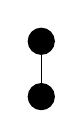
\begin{tikzpicture}
    \tikzset{level distance=20pt}
    \tikzset{sibling distance=72pt}
    \Tree [.\node[circle,draw,fill=black] {};  \node[circle,draw,fill=black] {}; ]
\end{tikzpicture}\end{center}
For higher derivatives it becomes more complicated to generate their form. Although not discussed thoroughly here, the Faa di Bruno formula using Bell functions can be used. Using this formula, we can generate the third derivative,
\begin{equation}
    \mathbf{y}^{\prime\prime\prime}\left(t\right) = \frac{d^2\mathbf{f}}{d^2\mathbf{y}}\left(\frac{d\mathbf{y}}{dt}\right)^2 + \frac{d\mathbf{f}}{d\mathbf{y}} \frac{d^2\mathbf{y}}{dt^2}.
\end{equation}
Here, we see that we need to do a substitution in two places for the derivatives of $\mathbf{y}$ with respect to time. Also, a separate tree is made for each term in the expression. Look at the first term only, we can substitute in Eq. \ref{eq:RT_D1} to get
\begin{equation}
    \frac{d^2\mathbf{f}}{d^2\mathbf{y}}\left(\frac{d\mathbf{y}}{dt}\right)^2.
\end{equation}
Because we substituted, we need to create a branch. Here, this will be a multinode branch since this term is squared. This rooted tree is depicted below.\\
\begin{center}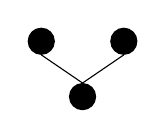
\begin{tikzpicture}[grow'=up]
    \tikzset{level distance=20pt}
    \tikzset{sibling distance=20pt}
    \Tree [.\node[circle,draw,fill=black] {}; [.\node[circle,draw,fill=black] {};] [.\node[circle,draw,fill=black] {}; ] ]
\end{tikzpicture}\end{center}
For the second term we substitute in Eq. \ref{eq:RT_D1} where we simply attach that 2-node single branch tree to the base tree of this equation. This rooted tree is shown below. \\
\begin{center}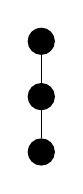
\begin{tikzpicture}
    \tikzset{level distance=20pt}
    \tikzset{sibling distance=72pt}
    \Tree [.\node[circle,draw,fill=black] {};  [.\node[circle,draw,fill=black] {}; \node[circle,draw,fill=black] {};]]
\end{tikzpicture}\end{center}
Finally, we can just summarize this third derivative example with the following equation:
\begin{equation}
    \mathbf{y}^{\prime\prime\prime}\left(t\right) = \frac{d^2\mathbf{f}}{d^2\mathbf{y}}\underbrace{\left(\frac{d\mathbf{y}}{dt}\right)^2}_{\mathrm{multi\,branch}} + \frac{d\mathbf{f}}{d\mathbf{y}} \underbrace{\frac{d\mathbf{f}}{d\mathbf{y}}\mathbf{f}\left[\mathbf{y}\left(t\right)\right]}
    _{\mathrm{single\,branch}}.
\end{equation}
Figure \ref{fig:RT} shows all the rooted trees up through 4th order.
\begin{figure}
  \centering
  
\begin{tikzpicture}
    \tikzstyle{every node}=[circle,draw,fill=black,text=white]
    \node {1};
  \end{tikzpicture} \hspace{1cm}
  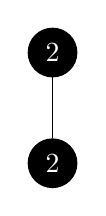
\begin{tikzpicture}
    \tikzset{level distance=40pt}
    \tikzset{sibling distance=72pt}
    \tikzstyle{every node}=[circle,draw,fill=black,text=white]
    \Tree [.\node {2};  \node {2}; ]
  \end{tikzpicture} \hspace{1cm}
  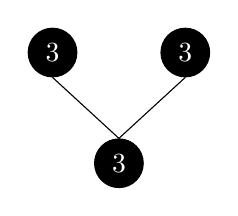
\begin{tikzpicture}[grow'=up]
    \tikzset{level distance=40pt}
    \tikzset{sibling distance=30pt}
    \tikzstyle{every node}=[circle,draw,fill=black,text=white]
    \Tree [.\node {3};  [.\node {3}; ] [.\node {3};] ]
  \end{tikzpicture} \hspace{1cm}
  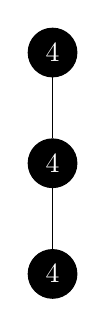
\begin{tikzpicture}[grow'=up]
    \tikzset{level distance=40pt}
    \tikzset{sibling distance=30pt}
    \tikzstyle{every node}=[circle,draw,fill=black,text=white]
    \Tree [.\node {4};  [.\node {4};  \node {4};] ]
  \end{tikzpicture} \hspace{1cm}
  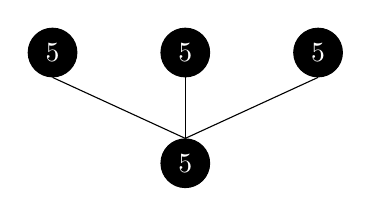
\begin{tikzpicture}[grow'=up]
    \tikzset{level distance=40pt}
    \tikzset{sibling distance=30pt}
    \tikzstyle{every node}=[circle,draw,fill=black,text=white]
    \Tree [.\node {5};  \node {5};  \node {5}; \node{5}; ]
  \end{tikzpicture}\hspace{1cm} 
  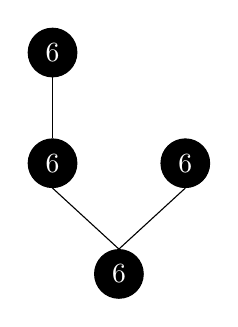
\begin{tikzpicture}[grow'=up]
    \tikzset{level distance=40pt}
    \tikzset{sibling distance=30pt}
    \tikzstyle{every node}=[circle,draw,fill=black,text=white]
    \Tree [.\node {6};  [.\node {6};  \node {6};] \node {6};  ]
  \end{tikzpicture} \hspace{1cm}
  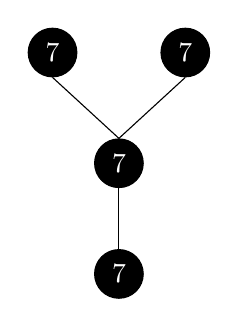
\begin{tikzpicture}[grow'=up]
    \tikzset{level distance=40pt}
    \tikzset{sibling distance=30pt}
    \tikzstyle{every node}=[circle,draw,fill=black,text=white]
    \Tree [.\node {7};  [.\node {7};  \node {7}; \node {7};]  ]
  \end{tikzpicture} \hspace{1cm}
  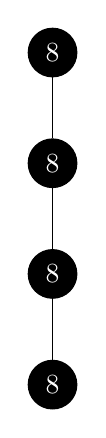
\begin{tikzpicture}[grow'=up]
    \tikzset{level distance=40pt}
    \tikzset{sibling distance=30pt}
    \tikzstyle{every node}=[circle,draw,fill=black,text=white]
    \Tree [.\node {8};  [.\node {8};  [.\node {8}; [.\node {8};]]] ]
  \end{tikzpicture}
\caption{Rooted trees for determining 4th order GRK coefficients.}
\label{fig:RT}
\end{figure}
The numbering of the trees is present to see the order of there equations. Note that the derivative order that the trees represent is the number of nodes. Using these rooted trees we can derive the order equations to solve for the GRK coefficients. We seek to construct equations that have the form
\begin{equation} \label{eq:RT_psi}
    \sum_i m_i \Psi_i\left(t\right) = \frac{1}{\Gamma\left(t\right)}.
\end{equation}
In this equation $m_i$ are the GRK coefficients listed in Eq. \eqref{eq:GRK_fund}. The parameter $\Psi\left(t\right)$ represents an equation derived from the rooted tree $t$ (not time). The last parameter is $\Gamma\left(t\right)$ and is defined as
\begin{equation}
    \Gamma\left(t\right) = \rho\left(t\right)\Gamma\left(t_1\right) ... \Gamma\left(t_m\right),
\end{equation}
where $\rho\left(t\right)$ is just the order, or number of nodes of tree $t$. This recursion is performed until all branches are removed and only node is left. Branches are removed by cutting off the root of the tree. Note this equation is recursive on $\Gamma$ and can get very complicated with complex rooted trees. To write equations, each branches are represented as parameters and are multiplied together. In GRK, if there is a single branch from node $j$ and it connects to node $k$ it is represented with a new parameter $\beta^\prime_{jk}$. However, if multiple branches are coming out of node $j$ and one of them connects to node $k$, this is represented with the already introduced GRK parameter $a_{jk}$. We make the following definitions:
\begin{equation}\label{eq:RT_simp}
    a_{i} = sum_j^{i-1} a_{ij} \qquad \beta^\prime_i = sum_j^i \beta^\prime_{ij} \qquad \beta^\prime_{ij} = a_{ij} + c_{ij}.
\end{equation}
Note that the limits of the summation are consistent with Eq. \eqref{eq:GRK_nonauto}. To show how this works we look at the first two rooted trees in Figure \ref{fig:RT}. Since we are constructing 4th order GRK, we always write every equation up through 4th order (defined as $s$). The first rooted tree has one node and the condition equation is simply
\begin{equation} \label{eq:RT_t1}
    \sum_i^s m_i = m_1 + m_2 + m_3 + m_4 = 1
\end{equation}
Here $\Gamma_{t_1}$ is simply just unity. The second rooted tree has one single branch. Therefore, its equation is
\begin{equation}
    \sum_i^s \mu_i\beta^\prime_{ij} = \frac{1}{2}. 
\end{equation}
For the summation of the highest branches, we can apply Eq. \eqref{eq:RT_simp} such that:
\begin{equation}
    \sum_i^s \mu_i\beta^\prime_i = \mu_1\beta^\prime_1 + \mu_2\beta^\prime_2 + \mu_3\beta^\prime_3 + \mu_4\beta^\prime_4 = \frac{1}{2}. 
\end{equation}
In Runge-Kutta methods, the problem is usually under constrained and we are free to choose some parameters. In GRK, Kaps and Rentrop and Kaps and Wanner define that
\begin{equation}
    c_{ii} \equiv \gamma ,
\end{equation}
which can be adjusted. They showed that this parameter has stability implications on the algorithm. Therefore, if this $\gamma$ parameter is known, we need to move it to the right hand side of the order equations. However, $\gamma$ does not explicitly show up. If we expand out the $\beta^\prime_i$ and noting that $a_{ii} = 0$ such that $\beta^\prime_{ii} = c_{ii} = \gamma$ we can write that
\begin{equation}
    \mu_1\beta^\prime_{11} + \mu_2\left(\beta^\prime_{21} + \beta^\prime_{22}\right) + \mu_3\left(\beta^\prime_{31} + \beta^\prime_{32} +\beta^\prime_{33} \right) + \mu_4\left(\beta^\prime_{41} + \beta^\prime_{42}+ \beta^\prime_{43} + \beta^\prime_{44}\right) = \frac{1}{2}
\end{equation}
and thus,
\begin{equation}
    \mu_1\gamma + \mu_2\left(\beta^\prime_{21} + \gamma\right) + \mu_3\left(\beta^\prime_{31} + \beta^\prime_{32} +\gamma \right) + \mu_4\left(\beta^\prime_{41} + \beta^\prime_{42}+ \beta^\prime_{43} + \gamma \right) = \frac{1}{2}.
\end{equation}
Moving this to the right hand side we can rewrite that
\begin{equation}
    \mu_2\beta^\prime_{21} + \mu_3\left(\beta^\prime_{31} + \beta^\prime_{32} \right) + \mu_4\left(\beta^\prime_{41} + \beta^\prime_{42}+ \beta^\prime_{43} \right) = \frac{1}{2} - \gamma\left(\mu_1 + \mu_2 + \mu_3 + \mu_4\right).
\end{equation}
If we look at the term in parenthesis on the right hand side of the equation it is the order equation of the first tree. Therefore, the right hand side will always have the equation of sub-trees as you remove branches. From the theory, this only applies to removing single branches. When no more single branches can be removed, the right hand side is complete. Therefore substituting the result of Eq. \eqref{eq:RT_t1} such that
\begin{equation}
    \mu_2\beta^\prime_{21} + \mu_3\left(\beta^\prime_{31} + \beta^\prime_{32} \right) + \mu_4\left(\beta^\prime_{41} + \beta^\prime_{42}+ \beta^\prime_{43} \right) = \frac{1}{2} - \gamma.
\end{equation}

Doing this manipulation can get cumbersome for each tree especially when they get complicated and there is an enormous amount of sub-trees. To make it easier to construct these equations, we redefine Eq. \eqref{eq:RT_psi} to
\begin{equation} \label{eq:RT_eq}
    \sum_i^s m_i \Phi\left(t\right) = \sum_{j\ge 0}^{\rho\left(t\right)-1} \left(-\gamma\right)^j \sum_{s \in V\left(t,j\right)} \frac{N\left(t,t^\prime\right)}{\Gamma\left(t^\prime\right)}.
\end{equation}
The notation of this equation is as follows:
\begin{itemize}
    \item $\rho\left(t\right)$ represents the order of the original tree,
    \item $j$ is a counter that represents the number of single branch nodes that have been removed from the original tree,
    \item $V\left(t,j\right)$ is a sub-tree $t^\prime$ that appears from the original tree $t$ by removing $j$ single branch nodes,
    \item $N\left(t,t^\prime\right)$ is the number of possibilities to obtain sub-tree $t^\prime$ by removing $j$ singly-branched nodes from the original tree $t$.
\end{itemize}
The second summation basically states that there may be multiple sub-trees that may be formed from the original tree by removing $j$ single branch nodes. This is just a convenient was of visually creating these order equations. Instead of $\Psi\left(t\right)$, we now have $\Phi\left(t\right)$.  The difference is that the $\beta^\prime_{ii}$ terms are no longer considered on the left hand side of the equation. Therefore, a new parameter $\beta$ is defined instead of $\beta^\prime$ such that
\begin{equation}\label{eq:simp2}
    \beta_i = \sum_j^{i-1} \beta_{ij} \qquad \beta_{ii} = 0 \qquad \beta_{ij} = a_{ij} + c_{ij}.
\end{equation}
If we consider the previous example for the second rooted tree, we can easily see that the relation is
\begin{align}
    \mu_2\beta_{21} + \mu_3\left(\beta_{31} + \beta_{32} \right) & + \mu_4\left(\beta_{41} + \beta_{42}+ \beta_{43} \right) \\ \nonumber & = \left(-\gamma\right)^0\cdot\left[\frac{N\left(t,t\right) = 1}{\Gamma\left(t\right) = 2\cdot 1}\right] + \left(-\gamma\right)^1\cdot\left[\frac{N\left(t,t^\prime\right) = 1}{\Gamma\left(t^\prime\right) = 1}\right]\\ \nonumber  & = \frac{1}{2} - \gamma .
\end{align}

Before moving on to defining each order equation for the rooted trees in Figure \ref{fig:RT}, we look at a more complicated tree to address some of the possible confusion. The tree is made up of 6 nodes shown below. \\
\begin{center}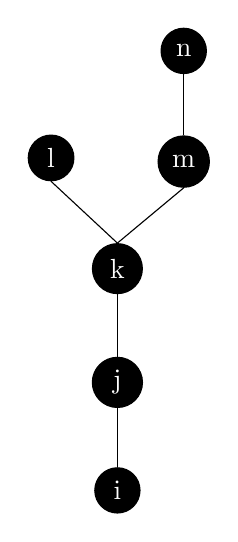
\begin{tikzpicture}[grow'=up]
    \tikzset{level distance=40pt}
    \tikzset{sibling distance=30pt}
    \tikzstyle{every node}=[circle,draw,fill=black,text=white]
    \Tree [.\node {i};  [.\node {j}; [.\node{k}; \node{l}; [.\node {m}; \node{n};]]]]
\end{tikzpicture}\end{center}
The first step is to define $\Phi_i\left(t\right)$ which can be determined by looking at the branch structure of the tree:
\begin{equation}    
    \Phi_i\left(t\right) = \beta_{ij}\beta_{jk}a_{k}a_{km}\beta_{m}
\end{equation}
Recall that the nodes on the extremities may be summed over which is why there is no $l$ or $n$ designation, rather there is a $k$ and $m$. Most of the work goes in to defining the right hand side of Eq. \eqref{eq:RT_eq}. To do this we must list all of the possible trees by removing single-branch nodes. The sub-trees are shown if Figure .
\begin{figure}
    \centering
  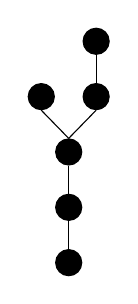
\begin{tikzpicture}[grow'=up]
    \tikzset{level distance=20pt}
    \tikzset{sibling distance=10pt}
    \tikzstyle{every node}=[circle,draw,fill=black,text=white]
    \Tree [.\node {};  [.\node {}; [.\node{}; \node{}; [.\node {}; \node{};]]]]
  \end{tikzpicture} \hspace{0.5cm}
  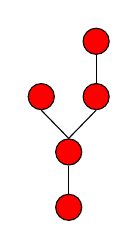
\begin{tikzpicture}[grow'=up]
    \tikzset{level distance=20pt}
    \tikzset{sibling distance=10pt}
    \tikzstyle{every node}=[circle,draw,fill=red,text=white]
    \Tree [.\node {}; [.\node{}; \node{}; [.\node {}; \node{};]]]
  \end{tikzpicture} \hspace{0.5cm}
  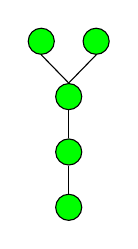
\begin{tikzpicture}[grow'=up]
    \tikzset{level distance=20pt}
    \tikzset{sibling distance=10pt}
    \tikzstyle{every node}=[circle,draw,fill=green,text=white]
    \Tree [.\node {};  [.\node {}; [.\node{}; \node{}; [.\node {};]]]]
  \end{tikzpicture}  \\ \vspace{1.0em}
  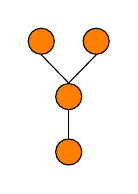
\begin{tikzpicture}[grow'=up]
    \tikzset{level distance=20pt}
    \tikzset{sibling distance=10pt}
    \tikzstyle{every node}=[circle,draw,fill=orange,text=white]
    \Tree [.\node {}; [.\node{}; \node{}; [.\node {};]]]
  \end{tikzpicture} \hspace{0.5cm}
  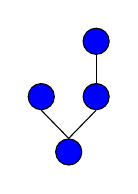
\begin{tikzpicture}[grow'=up]
    \tikzset{level distance=20pt}
    \tikzset{sibling distance=10pt}
    \tikzstyle{every node}=[circle,draw,fill=blue,text=white]
    \Tree [.\node{}; \node{}; [.\node {}; \node{};]]
  \end{tikzpicture} \hspace{0.5cm}
  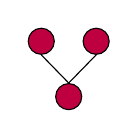
\begin{tikzpicture}[grow'=up]
    \tikzset{level distance=20pt}
    \tikzset{sibling distance=10pt}
    \tikzstyle{every node}=[circle,draw,fill=purple,text=white]
    \Tree [.\node{}; \node{}; [.\node {};]]
  \end{tikzpicture}
  \caption{Example of creating sub-trees from an original rooted tree shown in black.}
  \label{fig:RT_ex}
\end{figure}
The following list will give a description of how to calculate $N\left(t,t^\prime\right)$ and $\Gamma\left(t^\prime\right)$:
\begin{itemize}
    \item Black tree: This is the original tree. Therefore, there is only one way to form this so $N\left(t,t^\prime\right) = 1$. To determine $\Gamma\left(t^\prime\right)$, we successively cut off the root of the tree a multiply by the number of left over nodes. If trees become separated, they are treated as individual trees and their nodes are multiplied together. For the black tree, there is 6 nodes to begin with. If the root is cut off, there is still one tree and now there are 5 nodes. Again if the root of the tree is cut off there is still one tree and 4 nodes left. If we cut off the next root, two individual trees now exist, the first with 1 nodes and the second with 2 nodes. We finally cut off the root of the tree with 2 nodes left leaving it with one node. This is represented mathematically as $\Gamma\left(t^\prime\right) =  6\cdot 5\cdot 4\cdot 1\cdot 2\cdot 1$.
    \item {\color{red}Red tree}: This sub-tree can be achieved two different ways from the black tree. The first way is to remove the bottom-most single branch. The second way is to remove the single branch above that one. Therefore, $N\left(t,t^\prime\right) = 2$. Similar to the black tree, $\Gamma\left(t^\prime\right) =  5\cdot 4\cdot 1\cdot 2\cdot 1$.
    \item {\color{green}Green tree}: There is only 1 possibility of going from the black tree to this tree and it is to remove the top-most single branch. Therefore, $N\left(t,t^\prime\right) = 1$ and $\Gamma\left(t^\prime\right) =  5\cdot 4\cdot 3\cdot 1\cdot 1$.
    \item {\color{orange}Orange tree}: This tree is obtained by removing two single branches from the black tree. However, there are two possibilities similar to how the red tree was created. Therefore, $N\left(t,t^\prime\right) = 2$ and $\Gamma\left(t^\prime\right) =  4\cdot 3\cdot 1 \cdot 1$.
    \item {\color{blue}Blue tree}: This tree is obtained by removing the bottom two single branches from the black tree. There is one possibility so that $N\left(t,t^\prime\right) = 1$ and $\Gamma\left(t^\prime\right) =  4\cdot 1\cdot 2\cdot 1$.
    \item {\color{purple}Purple tree}: This is the final sub-tree that can be formed by removing single branches. There is only one possible way this is formed so $N\left(t,t^\prime\right) = 1$ and $\Gamma\left(t^\prime\right) =  3\cdot 1\cdot 1$.
\end{itemize}
Using all of this information, the order condition is
\begin{align}
    \sum_{i,j,k,m} m_{i}\beta_{ij}\beta_{jk}a_{k}a_{km}\beta_{m} = &  \frac{1}{240} - \frac{2\gamma}{40} - \frac{\gamma}{60} + \frac{2\gamma^2}{12} + \frac{1\gamma^2}{8} - \frac{\gamma^3}{3} \\ \nonumber 
      = & \frac{1}{240} - \frac{\gamma}{15} + \frac{7\gamma^2}{24} - \frac{\gamma^3}{3}.
\end{align}

\Subsubsection{4-th order GRK order equations}

By now, hopefully it is clear on how to construct these order equations. Returning to 4-th order GRK order equations, these can be constructed using Figure \ref{fig:RT}. The order equations listed below:
\begin{equation}
  \sum m_i = 1 = p_1\left(\gamma\right),
\end{equation}
\begin{equation}
  \sum m_i\beta_i = 1/2 - \gamma = p_2\left(\gamma\right),
\end{equation}
\begin{equation}
  \sum m_ia_i^2 = 1/3 = p_3\left(\gamma\right),
\end{equation}
\begin{equation}
  \sum m_i\beta_{ij}\beta_j = 1/6 - \gamma + \gamma^2 = p_4\left(\gamma\right),
\end{equation}
\begin{equation}
  \sum m_ia_i^3 = 1/4 = p_5\left(\gamma\right),
\end{equation}
\begin{equation}
  \sum m_ia_ia_{ij}\beta_j = 1/8 - \gamma/3 = p_6\left(\gamma\right),
\end{equation}
\begin{equation}
  \sum m_i\beta_{ij}a_j^2 = 1/12 - \gamma/3 = p_7\left(\gamma\right),
\end{equation}
\begin{equation}
  \sum m_i\beta_{ij}\beta_{jk}\beta_{k} = 1/24 - \gamma/2 + 3\gamma^2/2 - \gamma^3 = p_8\left(\gamma\right).
\end{equation}  
We can expand out the summations for each of these equations. They all respectively become:
\begin{equation}
   m_1 + m_2 + m_3 + m_4 = p_1\left(\gamma\right),
\end{equation}
\begin{equation}
   m_1\beta_1 + m_2\beta_2 + m_3\beta_3 + m_4\beta_4 = p_2\left(\gamma\right),
\end{equation}
\begin{equation}
   m_1a^2_1 + m_2a^2_2 + m_3a^2_3 + m_4a^2_4 = p_3\left(\gamma\right),
\end{equation}
\begin{equation}
   m_2\beta_{21}\beta_1 + m_3\beta_{31}\beta_1 + m_3\beta_{32}\beta_2 + m_4\beta_{41}\beta_1 + m_4\beta_{42}\beta_2 + m_4\beta_{43}\beta_3 = p_4\left(\gamma\right),
\end{equation}
\begin{equation}
   m_1a^3_1 + m_2a^3_2 + m_3a^3_3 + m_4a^3_4 = p_5\left(\gamma\right),
\end{equation}
\begin{equation}
   m_2a_2a_{21}\beta_1 + m_3a_3a_{31}\beta_1 + m_3a_3a_{32}\beta_2 + m_4a_4a_{41}\beta_1 + m_4a_4a_{42}\beta_2 + m_4a_4a_{43}\beta_3 = p_6\left(\gamma\right),
\end{equation}
\begin{equation}
   m_2\beta_{21}a_1^2 + m_3\beta_{31}a_1^2 + m_3\beta_{32}a_2^2 + m_4\beta_{41}a_1^2 + m_4\beta_{42}a_2^2 + m_4\beta_{43}a_3^2 = p_7\left(\gamma\right),
\end{equation}
\begin{equation}
   m_3\beta_{32}\beta_{21}\beta_1 + m_4\beta_{42}\beta_{21}\beta_1 + m_4\beta_{43}\beta_{31}\beta_1 + m_4\beta_{43}\beta_{32}\beta_2 = p_8\left(\gamma\right).
\end{equation}
The first numerical implementation of the 4-th order Rosenbrock GRK equations was accomplished by Kaps and Rentrop. They developed a 4 stage algorithm (4-th order) by only having to perform 3 derivative evaluations. This will be clearer in Section \ref{sec:impl}. What you see from these simultaneous equations is that there are far more unknowns than equations. Kaps and Rentrop were able to develop a set of coefficients where they were able to take  
\begin{equation}
       a_3 = a_4 \quad a_{41} = a_{31} \quad a_{42} = a_{32} \quad a_{43} = 0.
\end{equation}
This translates into only having to perform 1 Jacobian matrix/vector evaluation and 3 derivative vector evaluations at every time step. These simplifications can be used to simplify the simultaneous equations such that
\begin{equation}
   m_1 + m_2 + m_3 + m_4 = p_1\left(\gamma\right),
\end{equation}
\begin{equation}
   m_2\beta_2 + m_3\beta_3 + m_4\beta_4 = p_2\left(\gamma\right),
\end{equation}
\begin{equation}
   m_2a^2_2 + m_3a^2_3 + m_4a^2_3 = p_3\left(\gamma\right),
\end{equation}
\begin{equation}
   m_3\beta_{32}\beta_2 + m_4\beta_{42}\beta_2 + m_4\beta_{43}\beta_3 = p_4\left(\gamma\right),
\end{equation}
\begin{equation}
   m_2a^3_2 + m_3a^3_3 + m_4a^3_3 = p_5\left(\gamma\right),
\end{equation}
\begin{equation}
   m_3a_3a_{32}\beta_2 + m_4a_3a_{32}\beta_2 = p_6\left(\gamma\right),
\end{equation}
\begin{equation}
   m_3\beta_{32}a_2^2 + m_4\beta_{42}a_2^2 + m_4\beta_{43}a_3^2 = p_7\left(\gamma\right),
\end{equation}
\begin{equation}
   m_4\beta_{43}\beta_{32}\beta_2 = p_8\left(\gamma\right).
\end{equation}
The equation set has now been reduced to 8 equations with 14 unknowns. Feldberg noticed that with certain Runge-Kutta equations, estimation of lower order solutions is possible. It has been proven that an embedded third order solution can be calculated from a similar form of GRK equations where
\begin{equation}
    \hat{\mathbf{y}} = \hat{m}_1\mathbf{k}_1 + \hat{m}_2\mathbf{k}_2 + \hat{m}_3\mathbf{k}_3.
\end{equation}
We can use the rooted trees from Figure \ref{fig:RT} up to third order. The order equations are determined to be
\begin{equation}
     \hat{m}_1 + \hat{m}_2 + \hat{m}_3 = p_1\left(\gamma\right)
\end{equation}
\begin{equation}
     \hat{m}_2\beta_2 + \hat{m}_3\beta_3 = p_2\left(\gamma\right)
\end{equation}
\begin{equation}
     \hat{m}_2a^2_2 + \hat{m}_3a^2_3 = p_3\left(\gamma\right)
\end{equation}
\begin{equation}
     \hat{m}_3\beta_{32}\beta_2 = p_4\left(\gamma\right)
\end{equation}
Now, there are 12 equations with 17 unknowns. This allowed us to cut the deficit of equations by 1. Although not derived out thoroughly, additional constraint equations can be derived by matching higher order rooted trees.  And finally, as stated before, the parameter $\gamma$ is free to be chosen with stability implications. The last needed equations are listed below and discussed further in Kaps and Rentrop:
\begin{equation}
   a_2 = 2\gamma
\end{equation}
\begin{equation}
    a_3 = \left(1/5 - 1/4a_2\right)/\left(1/4 - 1/3a_2\right)
\end{equation}
\begin{equation}
   m_3 = 0
\end{equation}
\begin{equation}
   m_4\beta_{42}a_2^3 + m_4\beta_{43}a_3^3 = 1/20 - \gamma/4 = p_{14}\left(\gamma\right)
\end{equation}
\begin{equation}
   \gamma = \mathrm{free \,\, parmeter}
\end{equation}
Now we have 17 equations with 17 unknowns! Both Kaps--Rentrop and Shampine has developed suitable coefficient sets. The only parameter that defines the set of coefficients is $\gamma$. Once this parameter is set all of the simultaneous equations can be solved for the rest of the coefficients. Unfortunately, the 16 equations are not linear and there for nonlinear methods can be applied to solve for the coefficients. However, these equations can be broken up into smaller problems that are linear. The method to solve for the coefficients is detailed in Appendix \ref{app:order}. Instead of using the parameter $\hat{m}_i$ for the third order solution, we only need the truncation error for variable time stepping. Therefore, the difference of $m_i$ and $\hat{m}_i$ is usually reported and is denoted by $e_i$. The Kaps--Rentrop and Shampine set of coefficients as derived from the simultaneous equations presented here are listed in Table . The parameter $c_{ij}$ can be derived from $a_{ij}$ and $\beta_{ij}$ as discussed in Eq. \eqref{eq:simp2} and are also available. For completeness, the parameters $d_1$ and $b_i$ from Eq. \ref{eq:GRK_nonauto} are also listed. They are based off other coefficients defined in Eq. \ref{eq:GRK_bd}. Recall that to define $b_i$ the parameter $c_{ii}$ is present and is just $\gamma$. Note, there are 3 forms of the Rosenbrock equations in the literature where the order coefficients are different but related. We show one of these other forms in Section \ref{sec:impl}.
\begin{table}
\caption{4-th Order GRK Coefficients}
\label{tab:coefs}
\centering
\begin{tabular}{ccc}
\toprule
Coefficient & Kaps--Rentrop & Shampine \tabularnewline
\midrule
\midrule
$\gamma$ & 0.231 & 0.5 \tabularnewline
\midrule
$m_1$ & 2.174873716527329e-01 & 8/27 \tabularnewline
\midrule
$m_2$ & 4.862290379901194e-01 & 1/8 \tabularnewline
\midrule
$m_3$ & 0 & 0 \tabularnewline
\midrule
$m_4$ & 2.962835903571476e-01 & 125/216 \tabularnewline
\midrule
$a_{21}$ & 0.462 & 1 \tabularnewline
\midrule
$a_{31}$ & -8.156681683272238e-02 & 12/25 \tabularnewline
\midrule
$a_{32}$ &  9.617751501660557e-01 & 3/25 \tabularnewline
\midrule
$c_{21}$ & -2.706296677524429e-01 & -2 \tabularnewline
\midrule
$c_{31}$ &  3.112544832940969e-01 & 33/25 \tabularnewline
\midrule
$c_{32}$ &  8.524456284818460e-03 & 3/5 \tabularnewline
\midrule
$c_{41}$ &  2.828168320435299e-01 & -7/125 \tabularnewline
\midrule
$c_{42}$ & -4.579594832807246e-01 & -57/250 \tabularnewline
\midrule
$c_{43}$ & -1.112083333333333e-01 & -1/10 \tabularnewline
\midrule
$e_1 = m_1 - \hat{m}_1$ & 9.345758761520596e-01 & -8/27 \tabularnewline
\midrule
$e_2 = m_2 - \hat{m}_2$ & -1.289950083770920 & -1/6 \tabularnewline
\midrule
$e_3 = m_3 - \hat{m}_3$ & 5.909061726171296e-02 & -25/216 \tabularnewline
\midrule
$e_4 = m_4$ & 2.962835903571476e-01 & 125/216 \tabularnewline
\midrule
$d_1$ & 0 & 0 \tabularnewline
\midrule
$d_2$ & 0.462 & 1 \tabularnewline
\midrule
$d_3$ & 8.802083333333334e-01 & 3/5 \tabularnewline
\midrule
$d_4$ & 8.802083333333334e-01 & 3/5  \tabularnewline
\midrule
$b_1 = \gamma$ & 0.231 & 0.5 \tabularnewline
\midrule
$b_2$ & -3.962966775244289e-02 & -3/2 \tabularnewline
\midrule
$b_3$ & 5.507789395789153e-01 & 121/50 \tabularnewline
\midrule
$b_4$ & -5.535098457052796e-02 & 29/250 \tabularnewline
\bottomrule
\end{tabular}
\end{table}
The Kaps--Rentrop coefficient match very well with the coefficients they derived in their work. For Shampine's, it is more difficult as in his work his Rosenbrock equations are in a different for. However, in Section \ref{sec:impl} we will modify these coefficients to a numerically efficient form of the GRK equations and we can compare them to literature. Shampine notes that the Kaps--Rentrop parameters are barely stable and that the 3rd order embedded solution is not stable at infinity Shampine proves that both 4th order and 3rd order solutions are stable at infinity. Therefore, we will use Shampine's coefficient set for all of the analysis in this work.

\Subsection{Implementation of 4-th Order GRK Algorithm} \label{sec:impl}

Recall the nonautonomous form of the Rosenbrock equations given in Eq. \eqref{eq:GRK_nonauto}. To solve for $\mathbf{k}_i$ we move the $c_{ii} = \gamma$ term in the summation on the right hand side of the equation to the left hand side. The Rosenbrock equations now have the form
\begin{equation} \label{eq:impl_rb1}
    \left(\mathbb{I} - \gamma h \mathbb{J}\right)\mathbf{k}_{i} = h\mathbf{f} \left(t_n + d_ih,\mathbf{y}_n + \sum_{j=1}^{i-1}a_{ij}\mathbf{k}_{j}\right) 
                   + h\mathbb{J}\sum_{j=1}^{i-1} c_{ij}\mathbf{k}_{j}  + h^2b_i\frac{d\mathbf{f}}{dt}.
\end{equation}
Notice that now, the Jacobian matrix is on both sides of the equation. Since it is still on the right hand side, a lot of sparse matrix-vector products are required. This is numerically inefficient. To circumvent this, we can define a variable transformation such that
\begin{equation}
	\mathbf{k}^\prime_i=\sum_{j=1}^{i-1}c_{ij}\mathbf{k}_j + \gamma\mathbf{k}_i.
\end{equation}
When this is substituted into Eq. \ref{eq:impl_rb1}, the numerically efficient form of the Rosenbrock equations is obtained,
\begin{equation}
    \left[\mathbb{I}/\left(\gamma h\right) - \mathbb{J}\right]\mathbf{k}^\prime_{i} = \mathbf{f} \left(t_n + d_ih,\mathbf{y}_n + \sum_{j=1}^{i-1}a^\prime_{ij}\mathbf{k}^\prime_{j}\right) 
                   + \frac{1}{h}\sum_{j=1}^{i-1} c^\prime_{ij}\mathbf{k}^\prime_{j}  + hb_i\frac{d\mathbf{f}}{dt}.
\end{equation}
This procedure is outline in Numerical Recipes by Press et al. It is now observed that the Jacobian matrix is only on the left hand side of the equation. It is also shown that some of the GRK coefficient need to be redefined. This can be achieved by inspection of the different forms of the Rosenbrock equation. The detailed derivation of this conversion is in Appendix \ref{app:conv}. Scripts are also provided in the appendix to do this conversion very quickly. The results modified coefficients are shown in Table \ref{tab:ef_coefs}, similar to Table \ref{tab:coefs}. 
\begin{table}
\caption{4-th Order GRK Coefficients for Numerically Efficient Rosenbrock Equations}
\label{tab:ef_coefs}
\centering
\begin{tabular}{ccc}
\toprule
Coefficient & Kaps--Rentrop & Shampine \tabularnewline
\midrule
\midrule
$\gamma$ & 0.231 & 0.5 \tabularnewline
\midrule
$m^\prime_1$ &  3.957503746640767 & 19/9 \tabularnewline
\midrule
$m^\prime_2$ &  4.624892388363308 & 1/2 \tabularnewline
\midrule
$m^\prime_3$ & 6.174772638750108e-01 & 25/108 \tabularnewline
\midrule
$m^\prime_4$ &  1.282612945269037 & 125/108 \tabularnewline
\midrule
$a^\prime_{21}$ & 2.0 & 2.0 \tabularnewline
\midrule
$a^\prime_{31}$ & 4.524708207373113 & 48/25 \tabularnewline
\midrule
$a^\prime_{32}$ & 4.163528788597644  & 6/25 \tabularnewline
\midrule
$c^\prime_{21}$ & -5.071675338776314 & -8.0 \tabularnewline
\midrule
$c^\prime_{31}$ & 6.020152728650829 & 372/25 \tabularnewline
\midrule
$c^\prime_{32}$ & 1.597506846726722e-01 & 12/5  \tabularnewline
\midrule
$c^\prime_{41}$ & -1.856343618686086 & -112/125 \tabularnewline
\midrule
$c^\prime_{42}$ & -8.505380858179807 & -54/125 \tabularnewline
\midrule
$c^\prime_{43}$ & -2.084075136023187 & -2/5 \tabularnewline
\midrule
$e^\prime_1$ & -2.302155402933007 & 17/54 \tabularnewline
\midrule
$e^\prime_2$ & -3.073634485392629 & 7/36 \tabularnewline
\midrule
$e^\prime_3$ & 8.732808018045042e-01 & 0.0 \tabularnewline
\midrule
$e^\prime_4$ & 1.282612945269037 & 125/108 \tabularnewline
\midrule
$d_1$ & 0 & 0 \tabularnewline
\midrule
$d_2$ & 0.462 & 1 \tabularnewline
\midrule
$d_3$ & 8.802083333333334e-01 & 3/5 \tabularnewline
\midrule
$d_4$ & 8.802083333333334e-01 & 3/5  \tabularnewline
\midrule
$b_1 = \gamma$ & 0.231 & 0.5 \tabularnewline
\midrule
$b_2$ & -3.962966775244289e-02 & -3/2 \tabularnewline
\midrule
$b_3$ & 5.507789395789153e-01 & 121/50 \tabularnewline
\midrule
$b_4$ & -5.535098457052796e-02 & 29/250 \tabularnewline
\bottomrule
\end{tabular}
\end{table}
The 4-th order Rosenbrock equations to implement and solve at every attempted time step are given as
\begin{equation}
\left[1/\left(h\gamma\right) - \mathbb{J}\right]\mathbf{k}^\prime_1 = \mathbf{f}\left(t_n, \mathbf{y}_n\right) + hb_1\frac{d\mathbf{f}}{dt},
\end{equation}
\begin{equation}
    \left[1/\left(h\gamma\right) - \mathbb{J}\right]\mathbf{k}^\prime_2 = \mathbf{f}\left(t_n + d_2h, \mathbf{y}_n + a^\prime_{21}\mathbf{k}^\prime_1\right) + c^\prime_{21}\mathbf{k}^\prime_1/h + hb_2\frac{d\mathbf{f}}{dt},
\end{equation}
\begin{equation}
    \left[1/\left(h\gamma\right) - \mathbb{J}\right]\mathbf{k}^\prime_3 = \mathbf{f}\left(t_n + d_3h, \mathbf{y}_n + a^\prime_{31}\mathbf{k}^\prime_1 + a^\prime_{32}\mathbf{k}^\prime_2\right) + \left(c^\prime_{31}\mathbf{k}^\prime_1 + c^\prime_{32}\mathbf{k}^\prime_2\right)/h + hb_3\frac{d\mathbf{f}}{dt},
\end{equation}
\begin{equation}
    \left[1/\left(h\gamma\right) - \mathbb{J}\right]\mathbf{k}^\prime_4 = \mathbf{f}\left(t_n + d_3h, \mathbf{y}_n + a^\prime_{31}\mathbf{k}^\prime_1 + a^\prime_{32}\mathbf{k}^\prime_2\right) + \left(c^\prime_{41}\mathbf{k}^\prime_1 + c^\prime_{42}\mathbf{k}^\prime_2 + c^\prime_{43}\mathbf{k}^\prime_3\right)/h + hb_4\frac{d\mathbf{f}}{dt}.
\end{equation}
The solution at the end of time step is obtained with
\begin{equation}
   \mathbf{y}^{n+1} = \mathbf{y}^n + m^\prime_1\mathbf{k}^\prime_1 + m^\prime_2\mathbf{k}^\prime_2 + m^\prime_3\mathbf{k}^\prime_3 + m^\prime_4\mathbf{k}^\prime_4.
\end{equation}
From the equations, once can see that 4 linear solves are required, 1 Jacobian evaluation and 3 derivative vector evaluations at each time step. The user of the algorithm provides a Jacobian routine that evaluates $\mathbb{J}$ and $\frac{d\mathbf{f}}{dt}$ and a derivative routine that evaluations $\mathbf{f}$. An algorithm of this method is outlined in Algorithm \ref{alg:GRK}.
\begin{algorithm}
\centering
\caption{4-th Order GRK Algorithm}
\label{alg:GRK}
\begin{algorithmic}[1]
  \State Evaluate $\mathbf{f}_1$ and $\mathbb{J}\rightarrow$ {\color{red}You supply both routines for $\mathbf{f}$ and $\mathbb{J}$}
  \For{\# of trial timesteps}
    \State Construct left hand side matrix, $\mathbb{A} = \left[1/\left(h\gamma\right) - \mathbb{J}\right]$
    \State Construct first right hand side vector, $\mathbf{RHS}_1$
    \State Solve $\mathbb{A}\mathbf{k}_1=\mathbf{RHS}_1$
    \State Get intermediate $t$ and $\mathbf{y}$ and evaluate $\mathbf{f}_2$
    \State Construct first right hand side vector, $\mathbf{RHS}_2$
    \State Solve $\mathbb{A}\mathbf{k}_2=\mathbf{RHS}_2$
    \State Get intermediate $t$ and $\mathbf{y}$ and evaluate $\mathbf{f}_3$
    \State Construct first right hand side vector, $\mathbf{RHS}_3$
    \State Solve $\mathbb{A}\mathbf{k}_3=\mathbf{RHS}_3$
    \State Construct first right hand side vector, $\mathbf{RHS}_4$
    \State Solve $\mathbb{A}\mathbf{k}_4=\mathbf{RHS}_4$
    \State Get final estimate of $\mathbf{y}$ and truncation error, $\mathbf{T}$
    \State Accept or reject truncation error and get new timestep
  \EndFor
\end{algorithmic}
\end{algorithm}

\Subsection{Automated Time Step Size Adjustment} \label{sec:var_ts}

The last major part to discuss with 4-th order GRK is the ability to do variable time stepping. This ability comes for free when doing this algorithm since the third order solution coefficients are need to constrain the fourth order coefficients. This is known as embedded Fehlberg methods, where the truncation error between the 4-th and 3-rd order solutions is given by
\begin{equation}
    \mathbf{T} = \left| \mathbf{y} - \hat{\mathbf{y}} \right| = \sum_{i=1}^s e^\prime_i \mathbf{k}_i.
\end{equation}
The 4-th order GRK algorithm works specifically well for stiff systems. With any stiff set of equations, a the residual or errors must be scaled appropriately. Therefore, this truncation error must be scaled to see the relative importance of the errors. It is recommended to use
\begin{equation}
	\mathbf{y}_\mathrm{scale} = \mathrm{max}\left(\mathbf{C},\left|\mathbf{y}\right|\right).
\end{equation}
The vector $\mathbf{C}$ is used to control the relative error above some threshold. If all parameters are in nondimensional units, this parameter is recommended to be on the order of unity.

After scaling, the max error in this relative truncation error vector can be compared against some user-defined tolerance (usually around 1e-5 - 1e-4). If the max relative error is less than the specified tolerance, the time step is accepted. The next estimated time step is calculated with
\begin{equation}
	h_{n+1} = 0.9h_n\left(\frac{\epsilon_\mathrm{tol}}{e_{\mathrm{max}}}\right)^{\frac{1}{4}}.
\end{equation}
This new time step is accepted as long as it is below $1.5\times h_n$. Otherwise, $1.5\times h_n$ is used so that the time step doesn't grow out of control. Note, just because the current time step was accepted, it doesn't mean that the next time step will be larger. The 0.9 safety can yield a time step that is less to ensure that the next time step evaluation will be accepted. If the max relative error is greater than the specified tolerance, the time step is rejected and has to be re-tried. The time step is decreased by
\begin{equation}
	h_{n+1} = 0.9h_n\left(\frac{\epsilon_\mathrm{tol}}{e_{\mathrm{max}}}\right)^{\frac{1}{3}}.
\end{equation}
Note that if the new time step is below $0.5\times h_n$, this time step is used instead.

\Section{Point Kinetics Equations}

The simplest reactor physics model to apply GRK to is the Point Kinetics Equations (PKE). These equations are simple zero dimensional equations where the physics of the reactor are represented through simple parameters. The derivation of the PKE are described in Appendix \ref{app:pkes}. They are 
\begin{equation} \label{eq:pkeP}
\frac{d}{dt}P\left(t\right) = \frac{\rho\left(t\right)-\beta}{\Lambda}P\left(t\right) + \sum_i\lambda_iC_i\left(t\right)
\end{equation}
and
\begin{equation} \label{eq:pkeC}
\frac{d}{dt}C_i\left(t\right) = \frac{\beta_i}{\Lambda}P\left(t\right) - \lambda_iC_i\left(t\right).
\end{equation}
Using Equations \eqref{eq:pkeP} and \eqref{eq:pkeC} the derivative vector can be created as
\begin{equation}
\frac{d}{dt}\left[\begin{array}{c}
P\left(t\right) \\
C_i\left(t\right)
\end{array} \right] = \left[ \begin{array}{c}
\frac{\rho\left(t\right)-\beta}{\Lambda}P\left(t\right) + \sum_i\lambda_iC_i\left(t\right) \\
\frac{\beta_i}{\Lambda}P\left(t\right) - \lambda_iC_i\left(t\right)
\end{array}
\right].
\end{equation}
The corresponding Jacobian matrix for this model is written as 
\begin{equation}
\mathbb{J} = \left[ \begin{array}{ccccc}
\frac{\rho\left(t\right)-\beta}{\Lambda} & \lambda_1 & \lambda_i & \hdots & \lambda_I \\
\frac{\beta_1}{\Lambda} & -\lambda_1 \\
\frac{\beta_i}{\Lambda} & & -\lambda_i \\
\vdots & & & \ddots \\
\frac{\beta_I}{\Lambda} & & & & -\lambda_I \\
\end{array} \right]
\qquad
\frac{d\mathbf{f}}{dt} = \left[ \begin{array}{c} \frac{P\left(t\right)}{\Lambda}\frac{d\rho}{dt} \\
0 \\
0 \\
0 \\
0
\end{array} \right].
\end{equation}

This model was coded up and interfaced with the GRK solver. Input data used in this simulation is presented in Table \ref{tab:pk_input}.
\begin{table}
\caption{Input Values used for PKE Feedback Analysis}
\label{tab:pk_input}
\centering
\begin{tabular}{cc||cc}
\toprule 
Parameter & Value & Parameter & Value\tabularnewline
\midrule
\midrule 
$\beta_1$ & 0.000218 & $\lambda_1$ & 0.012467 1/s \tabularnewline
$\beta_2$ & 0.001023 & $\lambda_2$ & 0.028292 1/s \tabularnewline
$\beta_3$ & 0.000605 & $\lambda_3$ & 0.042524 1/s \tabularnewline
$\beta_4$ & 0.001310 & $\lambda_4$ & 0.133042 1/s \tabularnewline
$\beta_5$ & 0.002200 & $\lambda_5$ & 0.292467 1/s \tabularnewline
$\beta_6$ & 0.000600 & $\lambda_6$ & 0.666488 1/s \tabularnewline
$\beta_7$ & 0.000540 & $\lambda_7$ & 1.634781 1/s \tabularnewline
$\beta_8$ & 0.000152 & $\lambda_8$ & 3.554600 1/s \tabularnewline
$\Lambda$ & $5.902\times 10^6$ s & & \tabularnewline
\bottomrule
\end{tabular}
\end{table}
The simplest case to run is PKE with a constant reactivity insertion. Therefore, the derivative of the reactivity will be zero. The power shape from a 0.1\$ reactivity insertion is shown in Figure \ref{fig:pk_rho_const_power}. As expected, there is a prompt jump immediately in the power and then an asymptotic exponential increase persists.  It is also very important to look at the rate at which the power converges in time to confirm that the method is 4th order. A convergence plot is shown in Figure \ref{fig:pk_rho_const_order}.
\begin{figure} 
\centering \includegraphics[scale=1.00]{./figs/pk_rho_const_power.pdf}
\caption{PKE relative power from constant reactivity insertion.}
\label{fig:pk_rho_const_power}
\end{figure}
\begin{figure} 
\centering \includegraphics[scale=1.00]{./figs/pk_rho_const_order.pdf}
\caption{PKE temporal convergence rate for constant reactivity insertion.}
\label{fig:pk_rho_const_order}
\end{figure}
Two convergence rate results are shown in the plot. The first shows first order convergence of backward Euler and the second verifies 4th order convergence rate of the implemented GRK algorithm.  The reference was taken to be the GRK results at a time step of 1e-5 seconds at the end of the transient. It is also observed that the error in the GRK scheme is orders of magnitude less than backward Euler.

The next example for PKE is a case with a linear ramp reactivity insertion where 0.1\$ is inserted over 10 seconds. This is different than the last example in that there is now a constant $\frac{d\mathbf{f}}{dt}$ term. This term is known exactly and has the slope of the reactivity ramp in it. The results of this case are shown in Figure \ref{fig:pk_rho_ramp_power}. The power looks to be the correct shape for this transient. A convergence rate test was generated again. Again, the reference is a time step of 1e-5 seconds at the end of the transient.  The results, shown in Figure \ref{fig:pk_rho_ramp_order}, show that close to 4-th order is achieved as the time step is reduced. However, numerical precision error may start to occur around 1e-10\% difference and so 4-th order is never really observed.
\begin{figure} 
\centering \includegraphics[scale=1.00]{./figs/pk_rho_ramp_power.pdf}
\caption{PKE relative power from ramp reactivity insertion.}
\label{fig:pk_rho_ramp_power}
\end{figure}
\begin{figure} 
\centering \includegraphics[scale=1.00]{./figs/pk_rho_ramp_order.pdf}
\caption{PKE temporal convergence rate for constant reactivity insertion.}
\label{fig:pk_rho_ramp_order}
\end{figure}

\Subsection{Nordheim-Fuchs Model}

The simplest reactor physics example with nonlinear feedback is the Nordheim-Fuchs model (NFM). This model couples simplified point kinetics equations with an adiabatic heat up model. It assumes that the transient occurs very quickly such that there are no delayed neutron effects. Furthermore, feedback from Doppler effect occurs instantaneously in the fuel.  The coupled set of ordinary differential equations are as follows:
\begin{equation}
    \frac{d}{dt}P\left(t\right) = \frac{\rho\left(t\right)-\beta}{\Lambda}P\left(t\right)
\end{equation}
and
\begin{equation}
    \frac{d}{dt}T_f\left(t\right) = \frac{1}{m_fc_f}P\left(t\right).
\end{equation}
The Nordheim-Fuchs model allows for a step reactivity insertion and Doppler feedback in the fuel. The reactivity model is 
\begin{equation}
    \rho\left(t\right) = \rho_0 - \alpha_f\left[T_f\left(t\right) - T_{f,0}\right].
\end{equation}
This equation shows the nonlinearity of the system of equations. Therefore, the fuel temperature must be known to get the reactivity correct and to get the fuel temperature, the reactivity must be known. The GRK scheme accounts for some of this nonlinearity in its Jacobian. The derivative vector and Jacobian for this model is
\begin{equation}
    \frac{d}{dt}\left[\begin{array}{c}
                        P\left(t\right) \\
                        T_f\left(t\right)
                      \end{array}\right] =
                \left[\begin{array}{c}
                        \frac{\rho_0 - \alpha_f\left(T_f\left(t\right) - T_{f,0}\right) - \beta}{\Lambda}P\left(t\right) \\
                        \frac{1}{m_fc_f}P\left(t\right)
                      \end{array}\right]
\end{equation}
and
\begin{equation}
    \mathbb{J} = \left[\begin{array}{cc}
                         \frac{\rho_0 - \alpha_f\left(T_f\left(t\right) - T_{f,i}\right) - \beta}{\Lambda} & -\frac{\alpha_f}{\Lambda}P\left(t\right) \\
                         \frac{1}{m_fc_f} & 0
                       \end{array}\right]
     \qquad
     \frac{d\mathbf{f}}{dt} = \left[\begin{array}{c}
                        0 \\
                        0 \\
                        \vdots
                      \end{array}\right]
\end{equation}
What is important about the NFM is that it has an analytical solution. If we define parameter $\omega$ to be
\begin{equation}
	\omega = \frac{\rho_0-\beta}{\Lambda},
\end{equation}
then the time dependence of power, fuel temperature and reactivity are as follows:
\begin{equation}
	P\left(t\right) = \frac{\Lambda\omega^2m_fc_f}{2\alpha}\mathrm{sech}^2\left(\frac{\omega t}{2}\right),
\end{equation}
\begin{equation}
	T_f\left(t\right) = \frac{\Lambda\omega}{\alpha}\mathrm{tanh}\left(\frac{\omega t}{2}\right) + T_f\left(0\right)
\end{equation}
and
\begin{equation}
	\rho\left(t\right) = \rho\left(0\right) - \left(\rho_0 - \beta\right)\mathrm{tanh}\left(\frac{\omega t}{2}\right).
\end{equation}

Results from GRK are compared to this analytical model to verify that the code is accurate.  This comparison is depicted in Figure \ref{fig:nordheim_fuchs}.
\begin{figure} 
\centering \includegraphics[scale=1.00]{./figs/nordheimfuchs.pdf}
\caption{Comparison of GRK code to Nordheim Fuchs Model.}
\label{fig:nordheim_fuchs}
\end{figure}
From the results, it is observed that GRK does very well when comparing to NFM. For the first time, the time step used as a function of time is reported. More results with variable time step will be discussed in Sections \ref{sec:1D} and \ref{sec:2D}. Before the first time step, the user supplied the code with a 1e-5 second time step. The GRK variable time step algorithm quickly noticed that this was too fine and coarsened it to about 6.5e-5 seconds. This is held fairly constant as the transient progress until feedback begins to take over. The change in the flux rapidly becomes less and less and so the time step is allowed to coarsen. This occurs until the flux quickly drops once feedback dominates and it quickly returns to its previous steady value.

\Subsection{Point Kinetics with Feedback}

It is often questioned whether an algorithm retains its order of convergence when nonlinearities are present. The NFM presented in the previous section was extended to include delayed neutron effects, energy deposition to coolant, and heat transfer between fuel and coolant.  Coolant flow through the core is also simulated. The set of coupled equations used will be described below. Terms highlighted in {\color{red} red} represent parameters that are input into the model.  The equations are:
  \begin{itemize}
    \item Equation for power (parameters in {\color{red}red} are inputs):
  \end{itemize}
  \begin{equation}
    \frac{dP}{dt} = \frac{\overbrace{{\color{red}\rho_0\left(t\right)} - {\color{red}\alpha_f}\left[T_f\left(t\right) - T_{f,0}\right] - {\color{red}\alpha_c}\left[T_c\left(t\right) - 
    T_{c,0}\right]}^{\rho\left(t\right)} - {\color{red}{\beta}}}{{\color{red}\Lambda}}P\left(t\right) + \sum_i{\color{red}\lambda_i}C_i\left(t\right),
    \label{eq:pk_power}
  \end{equation}
    \begin{itemize}
    \item Equation for precursors:
  \end{itemize}
  \begin{equation}
    \frac{dC_i}{dt} = \frac{{\color{red}\beta_i}}{{\color{red}\Lambda}}P\left(t\right) - {\color{red}\lambda_i}C_i\left(t\right),
  \end{equation}
    \begin{itemize}
    \item Equation for fuel temperature ($\xi$ is coolant power deposition fraction):
  \end{itemize}
  \begin{equation}
    \frac{dT_f}{dt} = \frac{1-{\color{red}\xi}}{{\color{red}m_fc_f}}P\left(t\right) - \frac{\color{red}hA}{\color{red}m_fc_f}\left[T_f\left(t\right) - T_c\left(t\right)\right],
  \end{equation}
    \begin{itemize}
    \item Equation for coolant temperature:
  \end{itemize}
  \begin{equation}
    \frac{dT_c}{dt} = \frac{{\color{red}\xi}}{{\color{red}m_cc_c}}P\left(t\right) + \frac{\color{red}hA}{\color{red}m_cc_c}\left[T_f\left(t\right) - T_c\left(t\right)\right]
    - \frac{2\color{red}\dot{m}}{\color{red}m_c}\left[T_c\left(t\right) - {\color{red}T_{in}}\right].
    \label{eq:pk_temp}
  \end{equation}
In Eqs. \eqref{eq:pk_power}-\eqref{eq:pk_temp}, the input variables are defined as:
\begin{itemize}
	\item $\rho_0\left(t\right)$ - time dependent input reactivity
	\item $\alpha_f$ - fuel temperature coefficient of reactivity
	\item $\alpha_c$ - coolant temperature coefficient of reactivity
	\item $\beta$ - total delayed neutron fraction
	\item $\beta_i$ - delayed neutron fraction of precursor group $i$
	\item $\Lambda$ - prompt neutron lifetime
	\item $\lambda_i$ - decay constant of precursor group $i$
	\item $\xi$ energy deposition fraction directly into coolant
	\item $m_f$ mass of fuel
	\item $m_c$ mass of coolant
	\item $c_f$ specific heat capacity of fuel
	\item $c_c$ specific heat capacity of coolant
	\item $hA$ heat transfer rate from fuel to coolant
	\item $\dot{m}$ mass flow rate of coolant
	\item $T_{in}$ inlet coolant temperature
\end{itemize}
The above equations are then placed in a derivative vector in the GRK code. The Jacobian of this model is
  \begin{equation}
    \mathbb{J} = \left[
    \begin{array}{ccccc}
      \frac{{\color{red}\rho_0\left(t\right)} - {\color{red}\alpha_f}\left[T_f\left(t\right) - T_{f,0}\right] - {\color{red}\alpha_c}\left[T_c\left(t\right) - 
    T_{c,0}\right]- {\color{red}{\beta}}}{{\color{red}\Lambda}} & \color{red}\lambda_i & \hdots & \frac{-\color{red}\alpha_f}{\color{red}\Lambda}P\left(t\right) 
    & \frac{-\color{red}\alpha_c}{\color{red}\Lambda}P\left(t\right) \vspace{0.1cm}\\
    
    \frac{{\color{red}\beta_i}}{{\color{red}\Lambda}} & -{\color{red}\lambda_i} \\
    
    \vdots & & \ddots \\
    
    \frac{1-{\color{red}\xi}}{{\color{red}m_fc_f}} & & & -\frac{\color{red}hA}{\color{red}m_fc_f} & \frac{\color{red}hA}{\color{red}m_fc_f} \vspace{0.1cm} \\
    
    \frac{{\color{red}\xi}}{{\color{red}m_cc_c}} & & & \frac{\color{red}hA}{\color{red}m_cc_c} & -\frac{{\color{red}hA} + 2\color{red}\dot{m}c_c}{\color{red}m_cc_c}
    \end{array}\right]
  \end{equation}
and
  \begin{equation}
     \frac{d\mathbf{f}}{dt} = \left[\begin{array}{c}
                        \frac{d\color{red}\rho_0}{dt}\frac{P\left(t\right)}{\color{red}\Lambda} \\
                        0 \\
                        \vdots
                      \end{array}\right].
  \end{equation}
Using this model, a rod ejection is simulated where reactivity is inserted linearly to \$1.2 over 0.2 seconds and is held constant. We expect the power to quickly rise when the rod is ejected. However, due to temperature feedback in the fuel and coolant, this abrupt power increase will be halted and a new steady state will form. Tables \ref{tab:pk_input} and \ref{tab:pk_feedback_input} list all of the input variables used in this simulation. The initial power of the system is 5 MW. All of the other steady state values can be inferred by setting the derivatives in Eqs. \eqref{eq:pk_power}-\eqref{eq:pk_temp} to zero.
\begin{table}
\caption{Input Values used for PKE Feedback Analysis}
\label{tab:pk_feedback_input}
\centering
\begin{tabular}{cc||cc}
\toprule 
Parameter & Value & Parameter & Value\tabularnewline
\midrule
\midrule 
$\alpha_f$ & $2.5\times 10^{-5}$ 1/K & $\alpha_c$ & $25\times 10^{-5}$ 1/K \tabularnewline
\midrule 
$\xi$ & $0.05$ & $hA$ & $14633$ W \tabularnewline
\midrule 
$m_f$ & $148.3$ kg & $m_c$ & $20.4$ kg \tabularnewline
\midrule 
$c_f$ & $312$ J/kg-K & $c_c$ & $5827$ J/kg-K \tabularnewline
\midrule 
$\dot{m}$ & $24.1$ kg/s & $T_{in}$ & $559$ K \tabularnewline
\bottomrule
\end{tabular}
\end{table}

This transient was solved in the GRK code. Figure \ref{fig:pk_feedback_all} shows the results of the analysis.
\begin{figure} 
\centering \includegraphics[scale=1.00]{./figs/pk_feedback_all.pdf}
\caption{Transient results for PKE with feedback.}
\label{fig:pk_feedback_all}
\end{figure}
As expected the power quickly rose when the rod was ejected and was limited by the temperature feedback from fuel and coolant. A plot of reactivity is also shown in the figure. Two curves are present, where the first represents the forcing function of the rod ejecting. A linear ramp is present and then held after the rod is out of the core. The second reactivity curve shown is the actual reactivity of the system.  It shows the point in time where the reactivity feedbacks from fuel and coolant start to dominate the rod reactivity insertion. The transient settles back to a different steady state as shown in the power and temperature plots.  The fuel temperature has increased by 200 K from this transient.  Finally, the variable time step behavior is shown where it coarsens and refines as appropriate.

The convergence rate of the power at different values of time is presented in Figure \ref{fig:pk_feedback_order}.
\begin{figure}
\centering \includegraphics[scale=1.00]{./figs/pk_feedback_order.pdf}
\caption{Converge rate results for point kinetics with feedback present.}
\label{fig:pk_feedback_order}
\end{figure}
Looking at the results for 0.002 seconds, the convergence rate is nearly 4th order. However, taking the results at a later time of 0.09 seconds, the convergence rate is first order. Similarly at the end of the transient, the convergence rate remains first order. This is somewhat disconcerting since once we put nonlinear feedback in, we lose all benefit of this algorithm with respect to convergence rate. Another reason why this may occur is that there is a bug in this portion of the code, however none have been found to date.

\Section{1-D Spatial Kinetics no Feedback}\label{sec:1D}

Before analysis a 2-D reactor with local thermal feedback, significant upgrades need to made to a code. Therefore, a 1-D spatial kinetics code will be written and use basic operators to represent complex space and energy dependence such that moving to 2-D with feedback will happen naturally. With any reactor physics application, we start with the neutron balance equation. Here, we show it in 3-D multigroup steady state form over a Cartesian volume cell,
\begin{equation}
\label{eq:NBE}
\sum_{u \in x,y,z} \frac{\overline{J}^{u,g}_{l+1/2,m,n} - \overline{J}^{u,g}_{l-1/2,m,n}}{\Delta_l^u} + \overline\Sigma_{t_{l,m,n}}\overline{\overline{\phi}}_{l,m,n}^g = \sum_{h=1}^G\upsilon\overline\Sigma^{h\rightarrow g}_{s_{l,m,n}}\overline{\overline{\phi}}_{l,m,n}^h + \frac{\chi_{l,m,n}^g}{k}\sum_{h=1}^G\nu\overline\Sigma^{h}_{f_{l,m,n}} \overline{\overline{\phi}}_{l,m,n}^h.
\end{equation}
The notation used in Eq. \eqref{eq:NBE} is as follows:
\begin{itemize}
	\item $u$ - primary direction, either $x$, $y$ or $z$,
	\item $l$ - spatial index corresponding to direction $u$,
	\item $m$ and $n$ - spatial indices of transverse directions $v$ and $w$,
	\item $g$ - energy group
	\item $h$ - energy group (dented for outgoing groups during energy transfer)
	\item $\overline{J}^{u,g}_{l\pm1/2,m,n}$ - net neutron current in on positive/negative face $l\pm1/2$ in direction $u$ and group $g$,
	\item $\Delta^u_l$ is the length of the cell in direction $u$,
	\item $\overline\Sigma_{t_{l,m,n}}$ is the cell-averaged macroscopic total cross section,
	\item $\overline{\overline{\phi}}_{l,m,n}^g$ is the cell-averaged neutron flux,
	\item $\upsilon\overline\Sigma^{h\rightarrow g}_{s_{l,m,n}}$ is the cell-averaged macroscopic neutron production scattering cross section (includes n,$x$n reactions) transferring from group $h$ to group $g$,
	\item $\chi_{l,m,n}^g$ total fission emission spectrum into group $g$,
	\item $k$ is the core multiplication factor,
	\item $\nu\overline\Sigma^{h}_{f_{l,m,n}}$ is the macroscopic neutron production fission cross section.
\end{itemize}
 We will apply the diffusion approximation to relate neutron current to flux. This approximation known as Fick's Law is
 \begin{equation}
     \overline{J}^{u,g}_{l\pm1/2,m,n} = -D_{l,m,n}^g\left.\frac{d\overline{\phi}^g}{du}\right|_{l\pm 1/2,m,n},
 \end{equation}
where $D_{l,m,n}^g$ is the diffusion coefficient and $\overline{\phi}^g$ is the group $g$ neutron flux averaged over the transverse area in directions $v$ and $w$. This equation is then discretized using mesh-centered finite difference methods. The derivation of the subsequent equation is detailed thoroughly in Appendix \ref{app:fdm}. Relations are shown for two cases:
\begin{itemize}
	\item cell-to-cell coupling
	\begin{equation}
	    \overline{J}^{u,g}_{l\pm1/2,m,n} = \frac{2D_{l\pm1,m,n}^gD_{l,m,n}^g}{D_{l\pm1,m,n}^g\Delta_l^u + D_{l,m,n}^g\Delta_{l\pm1}^u}\left(\pm\overline{\overline{\phi}}_{l\pm1,m,n}^g\mp \overline{\overline{\phi}}_{l,m,n}^g\right),
	\end{equation}
	\item cell-to-boundary coupling
	\begin{equation}
	    \overline{J}^{u,g}_{l\pm1/2,m,n} = \pm\frac{2D_{l,m,n}^g\left(1 - \beta_{l\pm1/2,m,n}^g\right)}{4D_{l,m,n}^g\left(1 + \beta_{l\pm1/2,m,n}^g\right) + \left(1 - \beta_{l\pm1/2,m,n}^g\right)\Delta_l^u}\overline{\overline{\phi}}_{l,m,n}^g.
	\end{equation}
\end{itemize}
The only new parameter not defined in these equations is the surface albedo, $\beta_{l\pm1/2,m,n}^g$ which is the ratio of incoming to outgoing partial neutron current. Therefore for reflective boundary conditions the albedo is 1.0, zero incoming current it is 0.0 and for zero flux it is -1.0.

An neutron balance equation with diffusion approximation can be written for each cell and energy group creating a linear system of equations. In steady state form, these coupled system of equations can be represented in operator form as
\begin{equation}\label{eq:steady_oper}
    \mathbb{M}\boldsymbol{\Phi} = \frac{1}{k}\mathbb{F}\boldsymbol{\Phi},
\end{equation}
where $\mathbb{M}$ represents the loss of neutrons and $\mathbb{F}$ represents the production of neutrons from fission. Note, this equation is a generalized eigenvalue problem. Therefore a suitable eigenvalue solver must be available to solve for the steady state flux shape and multiplication factor $k$.

After getting the steady state values, the transient diffusion equations or spatial kinetics equations can be solved. We can write the neutron balance equation from Eq. \eqref{eq:NBE} in time-dependent form as
\begin{align}
\label{eq:time_NBE}
\left(\frac{1}{v}\right)_{l,m,n}^g\frac{\partial}{\partial t}\overline{\overline{\phi}}_{l,m,n}^g + \sum_{u \in x,y,z} \frac{\overline{J}^{u,g}_{l+1/2,m,n} - \overline{J}^{u,g}_{l-1/2,m,n}}{\Delta_l^u} + \overline\Sigma_{t_{l,m,n}}\overline{\overline{\phi}}_{l,m,n}^g  & = \sum_{h=1}^G\upsilon\overline\Sigma^{h\rightarrow g}_{s_{l,m,n}}\overline{\overline{\phi}}_{l,m,n}^h \\ + \frac{\chi_{l,m,n}^{p,g}\left(1-\beta\right)}{k}\sum_{h=1}^G\nu\overline\Sigma^{hg}_{f_{l,m,n}}  \overline{\overline{\phi}}_{l,m,n}^h + \sum_i\chi_{i_{l,m,n}}^{d,g}\lambda_i C_{i_{l,m,n}}\nonumber.
\end{align}
Note that in Eq. \eqref{eq:time_NBE} all of the macroscopic cross sections may be time-dependent. Since we added time dependence back, we must include the delayed neutron precursors, which have their own separate balance equation. This balance is shown as
\begin{equation}
    \frac{\partial}{\partial t}C_{i_{l,m,n}} = \frac{\beta_i}{k}\sum_{h=1}^G\nu\overline\Sigma^{hg}_{f_{l,m,n}} \overline{\overline{\phi}}_{l,m,n}^h - \lambda_iC_{i_{l,m,n}}.
\end{equation}
If we make some simple assumptions we can write this in similar operator form as above. The first assumption is that the delayed fission spectrum is independent of precursor groups and that it is equivalent to the prompt neutron spectrum. This assumption will be fine for the cases in this work, but may not be applicable to all problems. We also define a modified precursor concentration which makes them energy group dependent
\begin{equation}
    \widetilde{C}_{i_{l,m,n}}^g = \chi_{l,m,n}^g C_{i_{l,m,n}}. 
\end{equation}
Therefore the simplified spatial kinetics equations and precursor balance equations are
\begin{align}
    \left(\frac{1}{v}\right)_{l,m,n}^g\frac{\partial}{\partial t}\overline{\overline{\phi}}_{l,m,n}^g + \sum_{u \in x,y,z} \frac{\overline{J}^{u,g}_{l+1/2,m,n} - \overline{J}^{u,g}_{l-1/2,m,n}}{\Delta_l^u} + \overline\Sigma_{t_{l,m,n}}\overline{\overline{\phi}}_{l,m,n}^g  & = \sum_{h=1}^G\upsilon\overline\Sigma^{h\rightarrow g}_{s_{l,m,n}}\overline{\overline{\phi}}_{l,m,n}^h \\ + \frac{\chi_{l,m,n}^{g}\left(1-\beta\right)}{k}\sum_{h=1}^G\nu\overline\Sigma^{hg}_{f_{l,m,n}}  \overline{\overline{\phi}}_{l,m,n}^h + \sum_i\lambda_i \widetilde{C}_{i_{l,m,n}}^g\nonumber.
\end{align}
and
\begin{equation}
    \frac{\partial}{\partial t}\widetilde{C}_{i_{l,m,n}}^g = \frac{\chi_{l,m,n}^{g}\beta_i}{k}\sum_{h=1}^G\nu\overline\Sigma^{hg}_{f_{l,m,n}} \overline{\overline{\phi}}_{l,m,n}^h - \lambda_i\widetilde{C}_{i_{l,m,n}}^g.
\end{equation}

We can write these equations in operator notation similar to Eq. \eqref{eq:steady_oper},
\begin{equation}
    \mathrm{diag}\left(\boldsymbol{\frac{1}{v}}\right)\frac{d}{dt}\boldsymbol{\Phi} + \mathbb{M}\left(t\right)\boldsymbol{\Phi} = \frac{1-\beta}{k}\mathbb{F}\left(t\right)\boldsymbol{\Phi} + \mathbb{D}\widetilde{\boldsymbol{C}}
\end{equation}
and
\begin{equation} \label{eq:prec}
    \frac{d}{dt}\widetilde{\boldsymbol{C}} = \frac{\beta}{k}\mathbb{F}\left(t\right)\boldsymbol{\Phi} -  \mathrm{diag}\left\lbrace\boldsymbol{\lambda}\right\rbrace
    \widetilde{\boldsymbol{C}}.
\end{equation}
Here we have introduced a new operator, the decay operator $\mathbb{D}$. This operator performs the dot product of decay constants with all precursor groups of a certain spatial location and energy group. Also, the loss and production operators are shown with time dependence. 

After spatial discretization, the equation becomes an ordinary differential equation. This can be directly used in the GRK code. Note that the transient will be started off the steady state solution that includes $\boldsymbol{\Phi}$ and $k$.  The multiplication factor, which balances production and destruction of neutrons at steady state, must be held constant throughout the transient. The steady-state values of the modified precursor concentrations can be easily calculated by setting the temporal derivative in Eq. \eqref{eq:prec},
\begin{equation}
    \widetilde{\boldsymbol{C}} = \mathrm{diag}\left\lbrace\boldsymbol{\lambda}\right\rbrace^{-1}\frac{\beta}{k}\mathbb{F}\boldsymbol{\Phi}.
\end{equation}
The derivative vector for the GRK solution is given as
\begin{equation}\label{eq:1D_deriv}
    \frac{d}{dt}\left[\begin{array}{c}
    \boldsymbol{\Phi} \\ \widetilde{\boldsymbol{C}} \end{array}\right] = 
    \left[\begin{array}{c}
    \mathrm{diag}\left(\boldsymbol{\frac{1}{v}}\right)^{-1}\left[\frac{1-\beta}{k}\mathbb{F}\left(t\right) - \mathbb{M}\left(t\right)\right]\boldsymbol{\Phi} + \mathrm{diag}\left(\boldsymbol{\frac{1}{v}}\right)^{-1}\mathbb{D}\widetilde{\boldsymbol{C}} \\
    \frac{\beta}{k}\mathbb{F}\left(t\right)\boldsymbol{\Phi} -  \mathrm{diag}\left\lbrace\boldsymbol{\lambda}\right\rbrace
    \widetilde{\boldsymbol{C}}
    \end{array}\right]
\end{equation}
If there are $nx\times ny\times nz$ spatial points with $ng$ energy groups and $ni$ precursor groups, the size of the derivative vector is $\left(ni+1\right)\times ng\times nx\times ny\times nz$. The Jacobian matrix and vector an be created from this derivative vector. The Jacobian matrix is
\begin{equation}
    \mathbb{J} = \left[ \begin{array}{cc} 
    \mathrm{diag}\left(\boldsymbol{\frac{1}{v}}\right)^{-1}\left[\frac{1-\beta}{k}\mathbb{F}\left(t\right) - \mathbb{M}\left(t\right)\right] & \mathrm{diag}\left(\boldsymbol{\frac{1}{v}}\right)^{-1}\mathbb{D} \\
     \frac{\beta}{k}\mathbb{F}\left(t\right) & \mathrm{diag}\left\lbrace\boldsymbol{\lambda}\right\rbrace
    \end{array}\right].
\end{equation}
Lastly, if any of the properties change with time this derivative must be captured. It will be assumed that the only type of change to the reactor is from a rod being withdrawn and thus only the thermal group absorption cross section will be altered.  Therefore, thus Jacobian vector for this forcing function is
\begin{equation}
    \frac{d\mathbf{f}}{dt} = \left[ \begin{array}{c}
    \mathrm{diag}\left(\boldsymbol{\frac{1}{v}}\right)^{-1} \frac{d\mathbb{M}}{dt}\boldsymbol{\Phi} \\ \mathbf{0}
    \end{array}\right] = \left[ \begin{array}{c}
    \mathrm{diag}\left(\boldsymbol{\frac{1}{v}}\right)^{-1} \frac{d\boldsymbol{\Sigma}_a}{dt}\boldsymbol{\Phi} \\ \mathbf{0}
    \end{array}\right]
\end{equation}
Subroutines can be written to interface with the GRK code to create this derivative vector and Jacobian matrix/vector.

\Subsection{Results}

To test the 1-D spatial kinetics equations derived in the beginning of this section, a simple 1-D heterogeneous core was created. The arrangement of materials in this core is shown in Figure \ref{fig:1D_layout}. Each 1-D assembly is 10 cm thick and is subdivided even further to 1 cm nodes for the finite difference calculation.  
\input{./figs/1D_geometry.tex}
The 1-D core is surrounded by 30 cm of reflector and basically consists of one fuel type. The center 20 cm region of fuel is allowed to have a variable rod. The input parameters and material properties are in Tables \ref{tab:pk_input} and \ref{tab:1D_input}.
\begin{table}
\caption{Input Values used for 1-D Spatial Kinetics Analysis}
\label{tab:1D_input}
\centering
\begin{tabular}{ll||ll}
\toprule 
Parameter & Value & Parameter & Value\tabularnewline
\midrule
\midrule 
Fuel $D_1$ & 1.3 cm & Fuel $D_2$ & 0.5 cm \tabularnewline
Fuel $\Sigma_a^1$ & 0.0098 1/cm & Fuel $\Sigma_a^2$ & 0.114 1/cm \tabularnewline
Fuel $\nu\Sigma_f^1$ & 0.006 1/cm & Fuel $\nu\Sigma_f^2$ & 0.1950 1/cm \tabularnewline
Fuel $\Sigma_s^{1\rightarrow 2}$ & 0.022 1/cm \tabularnewline
Fuel $\chi_1$ & 1.0 & Fuel $\chi_2$ & 0.0 \tabularnewline
Reflector $D_1$ & 1.5 cm & Reflector $D_2$ & 0.5 cm \tabularnewline
Reflector $\Sigma_a^1$ & 0.0002 1/cm & Reflector $\Sigma_a^2$ & 0.02 1/cm \tabularnewline
Reflector $\Sigma_s^{1\rightarrow 2}$ & 0.032 1/cm \tabularnewline
Kinetics $v_1$ & $4.374\times 10^7$ cm/s & Kinetics $v_2$ & $4.374\times 10^5$ cm/s \tabularnewline
\bottomrule
\end{tabular}
\end{table}

The GRK code was executed with a 1e-4 variable time step relative tolerance and an inner solver tolerance of 1e-8. The transient problem described in the previous section was analyzed. Results of the power evolution during the transient are shown in Figure \ref{fig:1D_power}.
\begin{figure} 
\centering \includegraphics[scale=1.00]{./figs/1D_power.pdf}
\caption{Relative power behavior during rod withdrawl/insertion transient.}
\label{fig:1D_power}
\end{figure}
The shape of the power is as expected, when the rod is withdrawn, there is a steep increase in the power. When the rod is fully withdrawn there is an asymptotic increase in the power until the rod is reinserted. Eventually, the core starts to approach a new steady state. Since there is no feedback, we can't say anything about what relative power the core settles back out at since the flux in steady state form is just an eigenvector. The shapes however should be equivalent at the beginning and end of the transient. Thermal flux shapes are presented in Figure \ref{fig:1D_fluxes}, where it is observed that the shapes at the beginning and end of the transient are equivalent.
\begin{figure} 
\centering \includegraphics[scale=1.00]{./figs/1D_fluxes.pdf}
\caption{Thermal Flux distributions at rod in/rod out times during transient.}
\label{fig:1D_fluxes}
\end{figure}
Reflector peaks are also visible consistent with the physics.

The variable time step algorithm discussed in Section \ref{sec:var_ts} is applied to this problem. The initial time step guessed for this problem is 0.01 seconds. The results for the variable time step algorithm are shown in Figure \ref{fig:1D_time}. 
\begin{figure}
\centering \includegraphics[scale=1.00]{./figs/1D_time.pdf}
\caption{Variable time step results for 1-D spatial kinetics.}
\label{fig:1D_time}
\end{figure}
Two curves are shown on the plot. The first is the actual time step used from the variable time step algorithm. The second is the number of trials of time steps used in the algorithm before the truncation error acceptance criterion was met. Because the transient has no perturbation for the first two seconds, the time step quickly groups at the maximum rate. Once, the transient begins, the time step quickly reduces and the number of time step trials increases.  Note that the maximum number of trials is seven and it only occurs in a couple of places. Most of the time, it is observed that only one trial is needed and the time step predictor algorithm does well.  This is evident between two and three seconds where the time step is being reduced, but the number of trials is one. Therefore the number of time steps attempted is not much greater than the number of time steps actually used.  

\Section{2-D LRA Benchmark}\label{sec:2D}

The 2-D LRA BWR benchmark problem is a common test to verify a spatial kinetics solution. The core layout is shown in Figure \ref{fig:LRA_layout}.

\begin{figure}[htbp]
    \centering
    
    % these dimensions are determined in arrow_dimms.ods

    \def\scale{1.1}

    \def\latWidth{0.2808363589*\scale}
    
    \tikzset{Assembly/.style={
        inner sep=0pt,
        text width=\latWidth in,
        minimum size=\latWidth in,
        draw=black,
        align=center
        }
    }
    
    \def\matone{blue}
    \def\mattwo{blue!50}
    \def\matthree{red}
    \def\matfour{yellow}
    \def\matfive{green}
    \def\matsix{yellow!50!red}

    \scalebox{1.0}{

      \begin{tikzpicture}[x=1in,y=1in]
      
        % draw assembly row/column headers
        
        \draw[red, thick] ($(-5*\latWidth,7*\latWidth)$) node[above, anchor=south] {A} -- ($(-5*\latWidth,6*\latWidth)$);
        \draw[red, thick] ($(-4*\latWidth,7*\latWidth)$) node[above, anchor=south] {B} -- ($(-4*\latWidth,6*\latWidth)$);
        \draw[red, thick] ($(-3*\latWidth,7*\latWidth)$) node[above, anchor=south] {C} -- ($(-3*\latWidth,6*\latWidth)$);
        \draw[red, thick] ($(-2*\latWidth,7*\latWidth)$) node[above, anchor=south] {D} -- ($(-2*\latWidth,6*\latWidth)$);
        \draw[red, thick] ($(-1*\latWidth,7*\latWidth)$) node[above, anchor=south] {E} -- ($(-1*\latWidth,6*\latWidth)$);
        \draw[red, thick] ($(0*\latWidth,7*\latWidth)$) node[above, anchor=south] {F} -- ($(0*\latWidth,6*\latWidth)$);
        \draw[red, thick] ($(1*\latWidth,7*\latWidth)$) node[above, anchor=south] {G} -- ($(1*\latWidth,6*\latWidth)$);
        \draw[red, thick] ($(2*\latWidth,7*\latWidth)$) node[above, anchor=south] {H} -- ($(2*\latWidth,6*\latWidth)$);
        \draw[red, thick] ($(3*\latWidth,7*\latWidth)$) node[above, anchor=south] {J} -- ($(3*\latWidth,6*\latWidth)$);
        \draw[red, thick] ($(4*\latWidth,7*\latWidth)$) node[above, anchor=south] {K} -- ($(4*\latWidth,6*\latWidth)$);
        \draw[red, thick] ($(5*\latWidth,7*\latWidth)$) node[above, anchor=south] {L} -- ($(5*\latWidth,6*\latWidth)$);
        
        \begin{scope}[rotate=90]
          \draw[red, thick] ($(-5*\latWidth,7*\latWidth)$) node[left, anchor=east] {1} -- ($(-5*\latWidth,6*\latWidth)$);
          \draw[red, thick] ($(-4*\latWidth,7*\latWidth)$) node[left, anchor=east] {2} -- ($(-4*\latWidth,6*\latWidth)$);
          \draw[red, thick] ($(-3*\latWidth,7*\latWidth)$) node[left, anchor=east] {3} -- ($(-3*\latWidth,6*\latWidth)$);
          \draw[red, thick] ($(-2*\latWidth,7*\latWidth)$) node[left, anchor=east] {4} -- ($(-2*\latWidth,6*\latWidth)$);
          \draw[red, thick] ($(-1*\latWidth,7*\latWidth)$) node[left, anchor=east] {5} -- ($(-1*\latWidth,6*\latWidth)$);
          \draw[red, thick] ($(0*\latWidth,7*\latWidth)$) node[left, anchor=east] {6} -- ($(0*\latWidth,6*\latWidth)$);
          \draw[red, thick] ($(1*\latWidth,7*\latWidth)$) node[left, anchor=east] {7} -- ($(1*\latWidth,6*\latWidth)$);
          \draw[red, thick] ($(2*\latWidth,7*\latWidth)$) node[left, anchor=east] {8} -- ($(2*\latWidth,6*\latWidth)$);
          \draw[red, thick] ($(3*\latWidth,7*\latWidth)$) node[left, anchor=east] {9} -- ($(3*\latWidth,6*\latWidth)$);
          \draw[red, thick] ($(4*\latWidth,7*\latWidth)$) node[left, anchor=east] {10} -- ($(4*\latWidth,6*\latWidth)$);
          \draw[red, thick] ($(5*\latWidth,7*\latWidth)$) node[left, anchor=east] {11} -- ($(5*\latWidth,6*\latWidth)$);
        \end{scope}
        
        % draw fuel assembly nodes
        
        \node [Assembly, fill=\matfive]  at ($(-5*\latWidth,5*\latWidth)$)  {}; % A11
        \node [Assembly, fill=\matfive]  at ($(-4*\latWidth,5*\latWidth)$)  {}; % B11
        \node [Assembly, fill=\matfive]  at ($(-3*\latWidth,5*\latWidth)$)  {}; % C11
        \node [Assembly, fill=\matfive]  at ($(-2*\latWidth,5*\latWidth)$)  {}; % D11
        \node [Assembly, fill=\matfive]  at ($(-1*\latWidth,5*\latWidth)$)  {}; % E11
        \node [Assembly, fill=\matfive]  at ($( 0*\latWidth,5*\latWidth)$)  {}; % F11
        \node [Assembly, fill=\matfive]  at ($( 1*\latWidth,5*\latWidth)$)  {}; % G11
        \node [Assembly, fill=\matfive]  at ($( 2*\latWidth,5*\latWidth)$)  {}; % H11
        \node [Assembly, fill=\matfive]  at ($( 3*\latWidth,5*\latWidth)$)  {}; % J11
        \node [Assembly, fill=\matfive]  at ($( 4*\latWidth,5*\latWidth)$)  {}; % K11
        \node [Assembly, fill=\matfive]  at ($( 5*\latWidth,5*\latWidth)$)  {}; % L11

        \node [Assembly, fill=\matfive]  at ($(-5*\latWidth,4*\latWidth)$)  {}; % A10
        \node [Assembly, fill=\matfive]  at ($(-4*\latWidth,4*\latWidth)$)  {}; % B10
        \node [Assembly, fill=\matfive]  at ($(-3*\latWidth,4*\latWidth)$)  {}; % C10
        \node [Assembly, fill=\matfive]  at ($(-2*\latWidth,4*\latWidth)$)  {}; % D10
        \node [Assembly, fill=\matfive]  at ($(-1*\latWidth,4*\latWidth)$)  {}; % E10
        \node [Assembly, fill=\matfive]  at ($( 0*\latWidth,4*\latWidth)$)  {}; % F10
        \node [Assembly, fill=\matfive]  at ($( 1*\latWidth,4*\latWidth)$)  {}; % G10
        \node [Assembly, fill=\matfive]  at ($( 2*\latWidth,4*\latWidth)$)  {}; % H10
        \node [Assembly, fill=\matfive]  at ($( 3*\latWidth,4*\latWidth)$)  {}; % J10
        \node [Assembly, fill=\matfive]  at ($( 4*\latWidth,4*\latWidth)$)  {}; % K10
        \node [Assembly, fill=\matfive]  at ($( 5*\latWidth,4*\latWidth)$)  {}; % L10

        \node [Assembly, fill=\matthree] at ($(-5*\latWidth,3*\latWidth)$)  {};  % A9
        \node [Assembly, fill=\matthree] at ($(-4*\latWidth,3*\latWidth)$)  {};  % B9
        \node [Assembly, fill=\matthree] at ($(-3*\latWidth,3*\latWidth)$)  {};  % C9
        \node [Assembly, fill=\matthree] at ($(-2*\latWidth,3*\latWidth)$)  {};  % D9
        \node [Assembly, fill=\matthree] at ($(-1*\latWidth,3*\latWidth)$)  {};  % E9
        \node [Assembly, fill=\matthree] at ($( 0*\latWidth,3*\latWidth)$)  {};  % F9
        \node [Assembly, fill=\matthree] at ($( 1*\latWidth,3*\latWidth)$)  {};  % G9
        \node [Assembly, fill=\matfive]  at ($( 2*\latWidth,3*\latWidth)$)  {};  % H9
        \node [Assembly, fill=\matfive]  at ($( 3*\latWidth,3*\latWidth)$)  {};  % J9
        \node [Assembly, fill=\matfive]  at ($( 4*\latWidth,3*\latWidth)$)  {};  % K9
        \node [Assembly, fill=\matfive]  at ($( 5*\latWidth,3*\latWidth)$)  {};  % L9

        \node [Assembly, fill=\matthree] at ($(-5*\latWidth,2*\latWidth)$)  {};  % A8
        \node [Assembly, fill=\matthree] at ($(-4*\latWidth,2*\latWidth)$)  {};  % B8
        \node [Assembly, fill=\matthree] at ($(-3*\latWidth,2*\latWidth)$)  {};  % C8
        \node [Assembly, fill=\matthree] at ($(-2*\latWidth,2*\latWidth)$)  {};  % D8
        \node [Assembly, fill=\matthree] at ($(-1*\latWidth,2*\latWidth)$)  {};  % E8
        \node [Assembly, fill=\matthree] at ($( 0*\latWidth,2*\latWidth)$)  {};  % F8
        \node [Assembly, fill=\matthree] at ($( 1*\latWidth,2*\latWidth)$)  {};  % G8
        \node [Assembly, fill=\matfour]  at ($( 2*\latWidth,2*\latWidth)$)  {};  % H8
        \node [Assembly, fill=\matfive]  at ($( 3*\latWidth,2*\latWidth)$)  {};  % J8
        \node [Assembly, fill=\matfive]  at ($( 4*\latWidth,2*\latWidth)$)  {};  % K8
        \node [Assembly, fill=\matfive]  at ($( 5*\latWidth,2*\latWidth)$)  {};  % L8

        \node [Assembly, fill=\mattwo]   at ($(-5*\latWidth,1*\latWidth)$)  {};  % A7
        \node [Assembly, fill=\matone]   at ($(-4*\latWidth,1*\latWidth)$)  {};  % B7
        \node [Assembly, fill=\matone]   at ($(-3*\latWidth,1*\latWidth)$)  {};  % C7
        \node [Assembly, fill=\matone]   at ($(-2*\latWidth,1*\latWidth)$)  {};  % D7
        \node [Assembly, fill=\matone]   at ($(-1*\latWidth,1*\latWidth)$)  {};  % E7
        \node [Assembly, fill=\mattwo]   at ($( 0*\latWidth,1*\latWidth)$)  {};  % F7
        \node [Assembly, fill=\mattwo]   at ($( 1*\latWidth,1*\latWidth)$)  {};  % G7
        \node [Assembly, fill=\matsix]   at ($( 2*\latWidth,1*\latWidth)$)  {};  % H7
        \node [Assembly, fill=\matsix]   at ($( 3*\latWidth,1*\latWidth)$)  {};  % J7
        \node [Assembly, fill=\matfive]  at ($( 4*\latWidth,1*\latWidth)$)  {};  % K7
        \node [Assembly, fill=\matfive]  at ($( 5*\latWidth,1*\latWidth)$)  {};  % L7

        \node [Assembly, fill=\mattwo]   at ($(-5*\latWidth,0*\latWidth)$)  {};  % A6
        \node [Assembly, fill=\matone]   at ($(-4*\latWidth,0*\latWidth)$)  {};  % B6
        \node [Assembly, fill=\matone]   at ($(-3*\latWidth,0*\latWidth)$)  {};  % C6
        \node [Assembly, fill=\matone]   at ($(-2*\latWidth,0*\latWidth)$)  {};  % D6
        \node [Assembly, fill=\matone]   at ($(-1*\latWidth,0*\latWidth)$)  {};  % E6
        \node [Assembly, fill=\mattwo]   at ($( 0*\latWidth,0*\latWidth)$)  {};  % F6
        \node [Assembly, fill=\mattwo]   at ($( 1*\latWidth,0*\latWidth)$)  {};  % G6
        \node [Assembly, fill=\matsix]   at ($( 2*\latWidth,0*\latWidth)$)  {};  % H6
        \node [Assembly, fill=\matsix]   at ($( 3*\latWidth,0*\latWidth)$)  {};  % J6
        \node [Assembly, fill=\matfive]  at ($( 4*\latWidth,0*\latWidth)$)  {};  % K6
        \node [Assembly, fill=\matfive]  at ($( 5*\latWidth,0*\latWidth)$)  {};  % L6

        \node [Assembly, fill=\matone]   at ($(-5*\latWidth,-1*\latWidth)$) {};  % A5
        \node [Assembly, fill=\matone]   at ($(-4*\latWidth,-1*\latWidth)$) {};  % B5
        \node [Assembly, fill=\matone]   at ($(-3*\latWidth,-1*\latWidth)$) {};  % C5
        \node [Assembly, fill=\matone]   at ($(-2*\latWidth,-1*\latWidth)$) {};  % D5
        \node [Assembly, fill=\matone]   at ($(-1*\latWidth,-1*\latWidth)$) {};  % E5
        \node [Assembly, fill=\matone]   at ($( 0*\latWidth,-1*\latWidth)$) {};  % F5
        \node [Assembly, fill=\matone]   at ($( 1*\latWidth,-1*\latWidth)$) {};  % G5
        \node [Assembly, fill=\matthree] at ($( 2*\latWidth,-1*\latWidth)$) {};  % H5
        \node [Assembly, fill=\matthree] at ($( 3*\latWidth,-1*\latWidth)$) {};  % J5
        \node [Assembly, fill=\matfive]  at ($( 4*\latWidth,-1*\latWidth)$) {};  % K5
        \node [Assembly, fill=\matfive]  at ($( 5*\latWidth,-1*\latWidth)$) {};  % L5

        \node [Assembly, fill=\matone]   at ($(-5*\latWidth,-2*\latWidth)$) {};  % A4
        \node [Assembly, fill=\matone]   at ($(-4*\latWidth,-2*\latWidth)$) {};  % B4
        \node [Assembly, fill=\matone]   at ($(-3*\latWidth,-2*\latWidth)$) {};  % C4
        \node [Assembly, fill=\matone]   at ($(-2*\latWidth,-2*\latWidth)$) {};  % D4
        \node [Assembly, fill=\matone]   at ($(-1*\latWidth,-2*\latWidth)$) {};  % E4
        \node [Assembly, fill=\matone]   at ($( 0*\latWidth,-2*\latWidth)$) {};  % F4
        \node [Assembly, fill=\matone]   at ($( 1*\latWidth,-2*\latWidth)$) {};  % G4
        \node [Assembly, fill=\matthree] at ($( 2*\latWidth,-2*\latWidth)$) {};  % H4
        \node [Assembly, fill=\matthree] at ($( 3*\latWidth,-2*\latWidth)$) {};  % J4
        \node [Assembly, fill=\matfive]  at ($( 4*\latWidth,-2*\latWidth)$) {};  % K4
        \node [Assembly, fill=\matfive]  at ($( 5*\latWidth,-2*\latWidth)$) {};  % L4

        \node [Assembly, fill=\matone]   at ($(-5*\latWidth,-3*\latWidth)$) {};  % A3
        \node [Assembly, fill=\matone]   at ($(-4*\latWidth,-3*\latWidth)$) {};  % B3
        \node [Assembly, fill=\matone]   at ($(-3*\latWidth,-3*\latWidth)$) {};  % C3
        \node [Assembly, fill=\matone]   at ($(-2*\latWidth,-3*\latWidth)$) {};  % D3
        \node [Assembly, fill=\matone]   at ($(-1*\latWidth,-3*\latWidth)$) {};  % E3
        \node [Assembly, fill=\matone]   at ($( 0*\latWidth,-3*\latWidth)$) {};  % F3
        \node [Assembly, fill=\matone]   at ($( 1*\latWidth,-3*\latWidth)$) {};  % G3
        \node [Assembly, fill=\matthree] at ($( 2*\latWidth,-3*\latWidth)$) {};  % H3
        \node [Assembly, fill=\matthree] at ($( 3*\latWidth,-3*\latWidth)$) {};  % J3
        \node [Assembly, fill=\matfive]  at ($( 4*\latWidth,-3*\latWidth)$) {};  % K3
        \node [Assembly, fill=\matfive]  at ($( 5*\latWidth,-3*\latWidth)$) {};  % L3

        \node [Assembly, fill=\matone]   at ($(-5*\latWidth,-4*\latWidth)$) {};  % A2
        \node [Assembly, fill=\matone]   at ($(-4*\latWidth,-4*\latWidth)$) {};  % B2
        \node [Assembly, fill=\matone]   at ($(-3*\latWidth,-4*\latWidth)$) {};  % C2
        \node [Assembly, fill=\matone]   at ($(-2*\latWidth,-4*\latWidth)$) {};  % D2
        \node [Assembly, fill=\matone]   at ($(-1*\latWidth,-4*\latWidth)$) {};  % E2
        \node [Assembly, fill=\matone]   at ($( 0*\latWidth,-4*\latWidth)$) {};  % F2
        \node [Assembly, fill=\matone]   at ($( 1*\latWidth,-4*\latWidth)$) {};  % G2
        \node [Assembly, fill=\matthree] at ($( 2*\latWidth,-4*\latWidth)$) {};  % H2
        \node [Assembly, fill=\matthree] at ($( 3*\latWidth,-4*\latWidth)$) {};  % J2
        \node [Assembly, fill=\matfive]  at ($( 4*\latWidth,-4*\latWidth)$) {};  % K2
        \node [Assembly, fill=\matfive]  at ($( 5*\latWidth,-4*\latWidth)$) {};  % L2

        \node [Assembly, fill=\mattwo]   at ($(-5*\latWidth,-5*\latWidth)$) {};  % A1
        \node [Assembly, fill=\matone]   at ($(-4*\latWidth,-5*\latWidth)$) {};  % B1
        \node [Assembly, fill=\matone]   at ($(-3*\latWidth,-5*\latWidth)$) {};  % C1
        \node [Assembly, fill=\matone]   at ($(-2*\latWidth,-5*\latWidth)$) {};  % D1
        \node [Assembly, fill=\matone]   at ($(-1*\latWidth,-5*\latWidth)$) {};  % E1
        \node [Assembly, fill=\mattwo]   at ($( 0*\latWidth,-5*\latWidth)$) {};  % F1
        \node [Assembly, fill=\mattwo]   at ($( 1*\latWidth,-5*\latWidth)$) {};  % G1
        \node [Assembly, fill=\matthree] at ($( 2*\latWidth,-5*\latWidth)$) {};  % H1
        \node [Assembly, fill=\matthree] at ($( 3*\latWidth,-5*\latWidth)$) {};  % J1
        \node [Assembly, fill=\matfive]  at ($( 4*\latWidth,-5*\latWidth)$) {};  % K1
        \node [Assembly, fill=\matfive]  at ($( 5*\latWidth,-5*\latWidth)$) {}; `% L1

      \end{tikzpicture}
    }
    
    % make the legend
    \begin{tikzpicture}
      \matrix [matrix of nodes]
          {
              \node [Assembly, fill=\matone, text=white] at (0,0) {1}; & Fuel 1, blade in~~~ & 
              \node [Assembly, fill=\mattwo] at (0,0) {2}; & Fuel 1, blade out~~ &
              \node [Assembly, fill=\matthree] at (0,0) {3}; & Fuel 2, blade in~~~ \\
              \node [Assembly, fill=\matfour] at (0,0) {4}; & Fuel 2, blade out~~~ & 
              \node [Assembly, fill=\matsix] at (0,0) {R}; & Fuel 2, blade in/out~~~&
              \node [Assembly, fill=\matfive] at (0,0) {5}; & Reflector~~\\ 
          };
    \end{tikzpicture}

    \caption{Layout of 2-D LRA Benchmark \label{fig:LRA_layout}}
\end{figure}


The core is composed of two fuel types each having a rod in and rod out configuration. In addition there is a sizeable reflector placed around the core. Fuel assemblies are created by forming 15x15 cm boxes. Highlighted in orange in Figure \ref{fig:LRA_layout} is a 2x2 block of assemblies for Fuel 2 that the control blade can be manipulated. In 2-D the thermal absorption cross section is just changed to simulate a 3-D blade drop. Material specifications are listed in Table \ref{tab:LRA_mats}.
\begin{table}
\centering
\caption{Material Specification for LRA Benchmark}
\label{tab:LRA_mats}
\begin{tabular}{ccccccc}
\toprule 
Region & Material & $g$ & $D_{g}\,\left[\mathrm{cm}\right]$ & $\Sigma_{a}^{g}\,\left[\mathrm{cm}^{-1}\right]$ & $\nu\Sigma_{f}^{g}\,\left[\mathrm{cm}^{-1}\right]$ & $\Sigma_{s}^{1\rightarrow2}\,\left[\mathrm{cm}^{-1}\right]$\tabularnewline
\midrule
\midrule 
\multirow{2}{*}{1} & Fuel 1, & 1 & 1.255 & 0.008252 & 0.004602 & 0.02533\tabularnewline
\cmidrule{2-7} 
 & blade in & 2 & 0.211 & 0.1003 & 0.1091 & \tabularnewline
\midrule 
\multirow{2}{*}{2} & Fuel 1, & 1 & 1.268 & 0.007181 & 0.004609 & 0.02767\tabularnewline
\cmidrule{2-7} 
 & blade out & 2 & 0.1902 & 0.07047 & 0.08675 & \tabularnewline
\midrule 
\multirow{2}{*}{3, R} & Fuel 2, & 1 & 1.259 & 0.008002 & 0.004663 & 0.02617\tabularnewline
\cmidrule{2-7} 
 & blade in & 2 & 0.2091 & 0.08344 & 0.1021 & \tabularnewline
\midrule 
\multirow{2}{*}{4} & Fuel 2, & 1 & 1.259 & 0.008002 & 0.004663 & 0.02617\tabularnewline
\cmidrule{2-7} 
 & blade out & 2 & 0.2091 & 0.073324 & 0.1021 & \tabularnewline
\midrule 
\multirow{2}{*}{5} & Reflector & 1 & 1.257 & 0.0006034 & 0 & 0.04754\tabularnewline
\cmidrule{2-7} 
 &  & 2 & 0.1592 & 0.01911 & 0 & \tabularnewline
\bottomrule
\end{tabular} 
\end{table}
The change in thermal absorption cross section in region 3/4 affected by control blade motion is given piecewise as
\begin{equation}\label{eq:LRA_xsrod}
    \Sigma_{a,R}^2\left(t\right) = \left\lbrace \begin{array}{cc} \Sigma_{a,3}^2\left(0\right)\cdot\left(1 -0.0606184\left[\mathrm{s}^{-1}\right]\cdot t \right) & \mathrm{if}\,t\le 2\mathrm{s} \\
    \Sigma_{a,3}^2\left(0\right)\cdot\left(1 -0.0606184\left[\mathrm{s}^{-1}\right]\cdot 2\left[\mathrm{s}\right] \right) & \mathrm{if}\,t > 2\mathrm{s} \end{array}\right. .
\end{equation}
In every local fine mesh location in the diffusion mesh, local thermal feedback is present affecting fast group absorption cross sections. Doppler feedback is incorporated in the following expression
\begin{equation}\label{eq:LRA_xstemp}
    \Sigma_a^1\left(T\right) = \Sigma_a^1\left(T_0\right)\left[1 + \gamma\left(\sqrt{T} - \sqrt{T_0}\right)\right],
\end{equation}
where $\gamma$ is defined in Table \ref{tab:LRA_params}. To compute temperatures an adiabatic heat up model is used given by
\begin{equation}\label{eq:Temp}
    \frac{\partial}{\partial t} T\left(t,\vec{r}\right) = \alpha\sum_h\Sigma_f^h\phi^h\left(t,\vec{r}\right),
\end{equation}
where $\alpha$ is given in Table \ref{tab:LRA_params}. Finally all normalizations are to core average power density which is related to fission density with
\begin{equation}\label{eq:Pdens}
    P\left(t,\vec{r}\right) = \kappa\sum_h\Sigma_f^h\phi^h\left(t,\vec{r}\right),
\end{equation}
where $kappa$ can be found in Table \ref{tab:LRA_params}. 
\begin{table}
\centering
\caption{Addition Parameters for LRA Benchmark}
\label{tab:LRA_params}
\begin{tabular}{cc||cc}
\toprule 
Parameter & Value & Parameter & Value\tabularnewline
\midrule
\midrule 
$v_{1}$ & $3.0\times10^{7}$ cm/s & $v_{2}$ & $3.0\times10^{5}$ cm/s\tabularnewline
\midrule 
$\beta_{1}$ & 0.0054 & $\beta_{2}$ & 0.001087\tabularnewline
\midrule 
$\lambda_{1}$ & 0.0654 & $\lambda_{2}$ & 1.35\tabularnewline
\midrule 
$\nu$ & 2.43 neutrons/fission & $\alpha$ & $3.83\times10^{-11}\,\mathrm{K\cdot cm^{3}}$\tabularnewline
\midrule 
$\gamma$  & $3.034\times10^{-3}\,\mathrm{K\cdot cm^{3}}$ & $\kappa$  & $3.204\times10^{-11}\,\mathrm{J/fission}$\tabularnewline
\midrule 
$B_{z}^{2}$ & $1.0\times10^{-4}\,\mathrm{cm^{-2}}$ &  & \tabularnewline
\bottomrule
\end{tabular}
\end{table}
The initial core power density is
\begin{equation}
    \overline{P}\left(0\right) = 1.0 \times 10^{-6}\,\mathrm{W/cm^3},
\end{equation}
where core average power density and temperature are given as
\begin{equation}\label{eq:aveP}
    \overline{P}\left(t\right) = \frac{\int_{V_f}d^3rP\left(t,\vec{r}\right)}{V_f}
\end{equation}
and
\begin{equation}
    \overline{T}\left(t\right) = \frac{\int_{V_f}d^3rT\left(t,\vec{r}\right)}{V_f}.
\end{equation}
These integrals are only over the fueled region of the LRA BWR model. Once the steady state eigenvalue and spatial group flux distribution are determined, these fluxes can be scaled up the specified power density.  This can be accomplished by multiplying all of the flux eigenvector by a constant which is the ratio of the desired power density to the power density computed with Eqs. \eqref{eq:Pdens} and \eqref{eq:aveP}. At the start of the transient, the core is at a uniform temperature of 300 K.

Although this is a 2-D problem, equations from Section \ref{sec:1D} can be extended with relative ease. The fact that we have added a dimension to the problem will be hidden in the operators. Therefore, the only element that we have to add to the 1-D equation set from Eq. \eqref{eq:1D_deriv} is the description of temperatures shown in continuous form in Eq. \eqref{eq:Temp}. The derivative vector becomes
\begin{equation}\label{eq:LRA_deriv}
    \frac{d}{dt}\left[\begin{array}{c}
    \boldsymbol{\Phi} \\ \widetilde{\boldsymbol{C}} \\ \boldsymbol{T}\end{array}\right] = 
    \left[\begin{array}{c}
    \mathrm{diag}\left(\boldsymbol{\frac{1}{v}}\right)^{-1}\left[\frac{1-\beta}{k}\mathbb{F} - \mathbb{M}\left(t\right)\right]\boldsymbol{\Phi} + \mathrm{diag}\left(\boldsymbol{\frac{1}{v}}\right)^{-1}\mathbb{D}\widetilde{\boldsymbol{C}} \\
    \frac{\beta}{k}\mathbb{F}\boldsymbol{\Phi} -  \mathrm{diag}\left\lbrace\boldsymbol{\lambda}\right\rbrace
    \widetilde{\boldsymbol{C}} \\
    \alpha \mathbb{F}^\prime\boldsymbol{\Phi}
    \end{array}\right].
\end{equation}
The operator notation for the temperature in Eq. \eqref{eq:LRA_deriv} is a little strange. The operator, $\mathbb{F}^\prime$ is a modified form of the fission source operator $\mathbb{F}$. The dimension of this matrix that represents this modified operator is just the spatial cells in the geometry by the product number of spatial points and groups. Therefore, it is a rectangular matrix. Each row consists of all group fission cross sections. The flux vector is then still consistent with other equations.  Doing this product, the summation over groups shown in Eq. \eqref{eq:Temp} will be correctly performed. Note that also in Eq. \eqref{eq:LRA_deriv} the only explicit time dependent term other than the state variables of the system is the operator $\mathbb{M}$ which will change due to "rod movement". An example of the structure of the Jacobian matrix is shown in Figure \ref{fig:jacobian}.
\begin{figure}
\centering 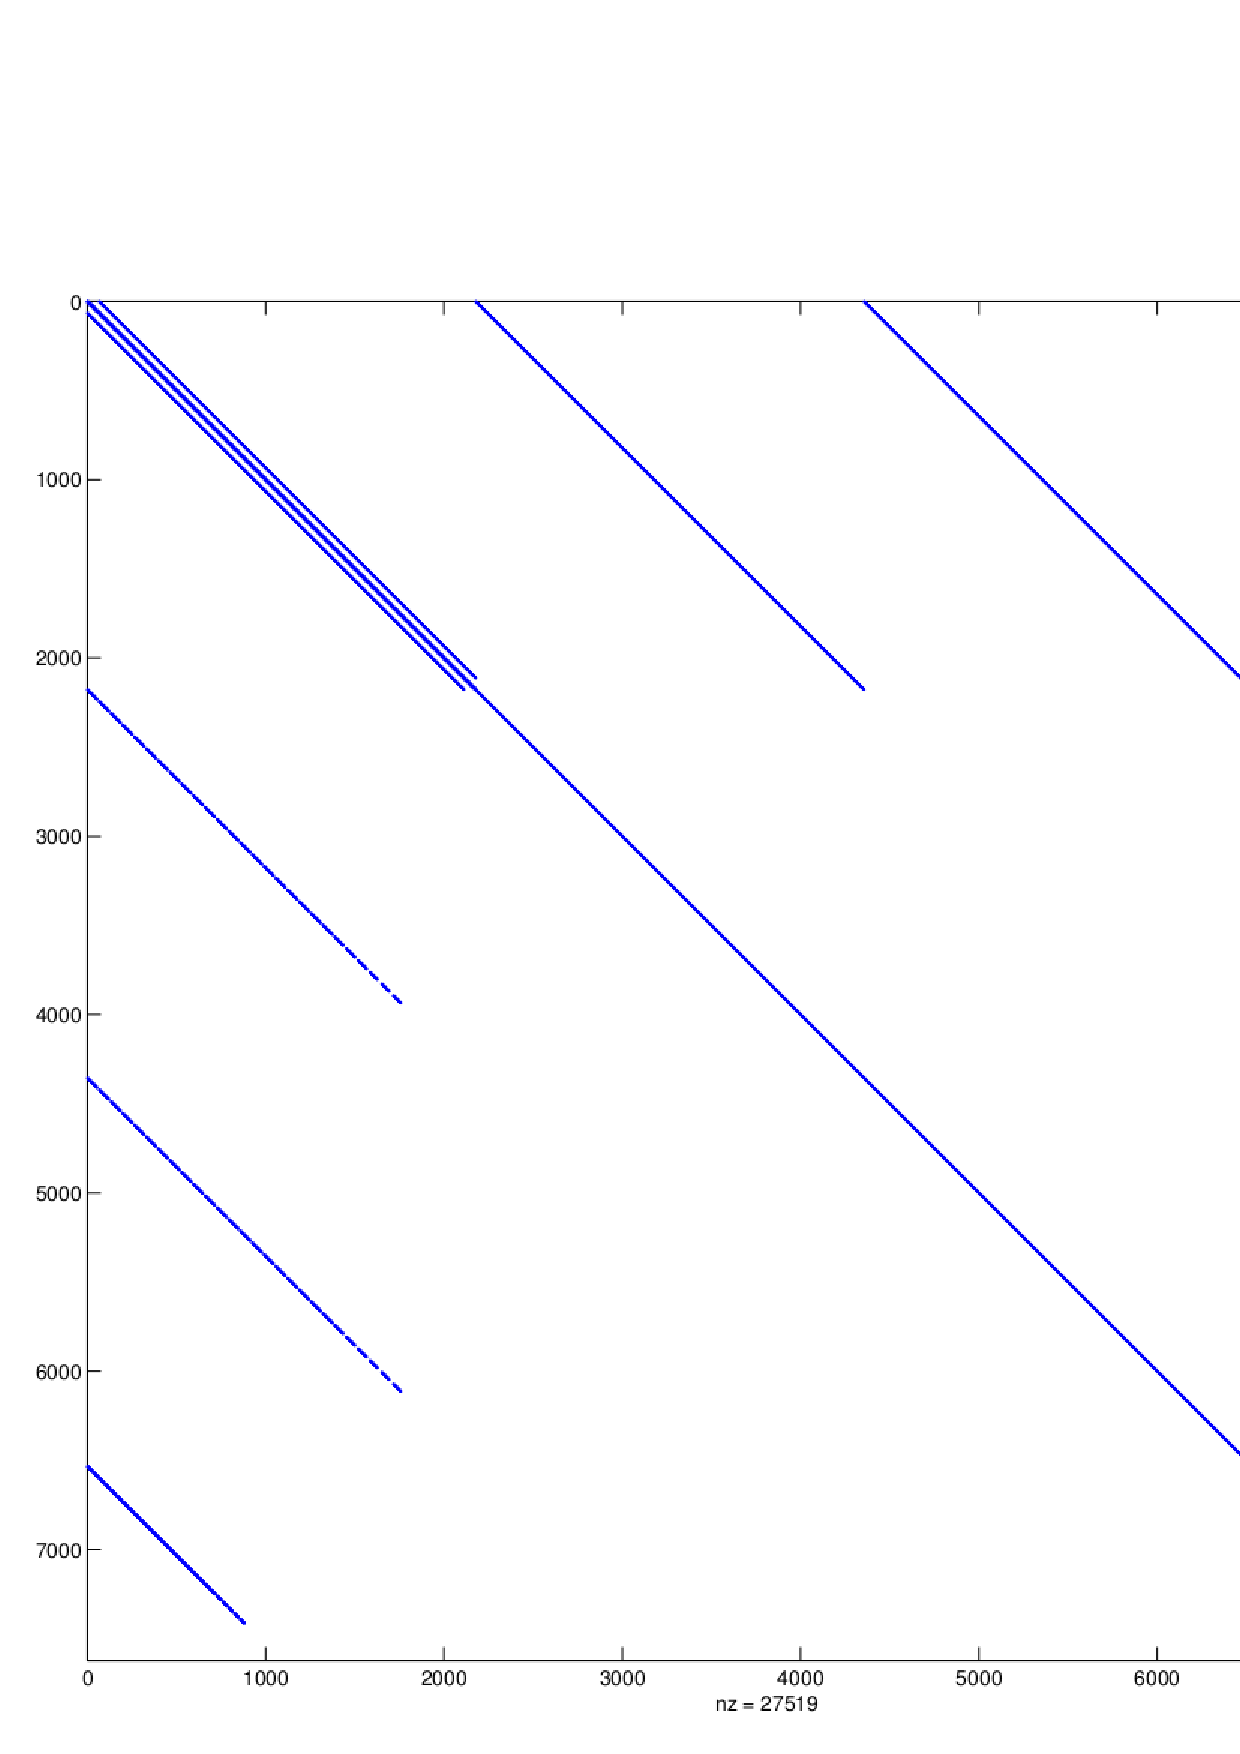
\includegraphics[scale=0.4]{./figs/jacobian.pdf}
\caption{Structure of Jacobian matrix for LRA benchmark.}
\label{fig:jacobian}
\end{figure}
The Jacobian matrix and vector in equation form are given as
\begin{equation} \label{eq:LRA_Jmat}
    \mathbb{J} = \left[ \begin{array}{ccc} 
    \mathrm{diag}\left(\boldsymbol{\frac{1}{v}}\right)^{-1}\left[\frac{1-\beta}{k}\mathbb{F}\left(t\right) - \mathbb{M}\left(t\right)\right] & \mathrm{diag}\left(\boldsymbol{\frac{1}{v}}\right)^{-1}\mathbb{D} & -\mathrm{diag}\left\lbrace\mathrm{diag}\left(\boldsymbol{\frac{1}{v}}\right)^{-1}\Gamma\left(\boldsymbol{T}\right)\right\rbrace\boldsymbol{\Phi}\\
     \frac{\beta}{k}\mathbb{F}\left(t\right) & \mathrm{diag}\left\lbrace\boldsymbol{\lambda}\right\rbrace \\
     \alpha\mathbb{F}^\prime
    \end{array}\right],
\end{equation}
and
\begin{equation}\label{eq:LRA_Jvec}
    \frac{d\mathbf{f}}{dt} = \left[ \begin{array}{c}
    \mathrm{diag}\left(\boldsymbol{\frac{1}{v}}\right)^{-1} \frac{d\mathbb{M}}{dt}\boldsymbol{\Phi} \\ \mathbf{0}
    \end{array}\right] = \left[ \begin{array}{c}
    \mathrm{diag}\left(\boldsymbol{\frac{1}{v}}\right)^{-1} \frac{d\boldsymbol{\Sigma}_a}{dt}\boldsymbol{\Phi} \\ \mathbf{0} \\ \mathbf{0}.
    \end{array}\right]
\end{equation}
In Eq. \eqref{eq:LRA_Jmat} the term $\gamma\left(\boldsymbol{T}\right)$  represents the derivative of the group 1 absorption cross section dependence on temperature in the operator $\mathbb{M}$. This term can be derived from Eq. \eqref{eq:LRA_xstemp} and is presented in scalar form as follows:
\begin{equation}
    \Gamma_i\left(T\right) = \frac{1}{2}\Sigma_a^1\gamma T^{-0.5}.
\end{equation}
Similarly in Eq. \eqref{eq:LRA_Jvec}, there is a derivative of absorption cross section with respect to time. This term appears due to the forcing function of the control rod movement. Fortunately, we are given an expression for this dependence in Eq. \eqref{eq:LRA_xsrod}. However, this term will only be nonzero in the region that has the control blade drop and only in group 2. This derivative is
\begin{equation}
    \frac{d}{dt}\Sigma_{a,R}^2\left(t\right) = \left\lbrace \begin{array}{cc} -\Sigma_{a,3}^2\left(0\right)\cdot 0.0606184\left[\mathrm{s}^{-1}\right] & \mathrm{if}\,t\le 2\mathrm{s} \\
    0 & \mathrm{if}\,t > 2\mathrm{s} \end{array}\right. .
\end{equation}
These models can be coded up and interfaced with the GRK solver as done with previous simulations. 

\Subsection{LRA Results}

Before the transient results are reported, the LRA benchmarks needs to be solved for a steady state eigenvalue and flux solution. Here, we investigate two spatial meshes, 15.0 and 1.5 cm. The 15.0 cm mesh corresponds to having one finite difference mesh per assembly, whereas for the 1.5 cm mesh, there will be ten. Table \ref{tab:LRA_eigs} shows the eigenvalue results and static control blade worth.
\begin{table}
\centering
\caption{Eigenvalue and Blade Worth Results}
\label{tab:LRA_eigs}
\begin{tabular}{ccc}
\toprule 
 & 15 cm mesh & 1.5 cm mesh\tabularnewline
\midrule
\midrule 
Blade in $k_{eff}$ & 1.003892 & 0.996283\tabularnewline
\midrule 
Blade out $k_{eff}$ & 1.028262 & 1.015192\tabularnewline
\midrule 
Blade worth $\left[\beta\right]$ & $\frac{1.028262-1.003892}{1.028262\cdot\beta}=3.65\beta$ & $\frac{1.015192-0.996283}{1.015192\cdot\beta}=2.87\beta$\tabularnewline
\midrule
\midrule
Reference $k_{eff}$ & 0.99636 & $\beta=0.006487$ \tabularnewline
\bottomrule
\end{tabular}
\end{table}
Normalized assembly power distributions for rodded and unrodded cases for both the 15 cm and 1.5 cm mesh are presented in Figures \ref{fig:LRA_15_rodin} -- \ref{fig:LRA_1.5_rodout}.These figures show how the relative assembly power distribution changes when the control blade is dropped. There is a large spike in the unrodded assemblies.  Also from these spatial plots, we can observe the errors from spatial discretization between 15cm and 1.5cm.
\input{./figs/LRA_15_rodin0.tex}
\input{./figs/LRA_1.5_rodin0.tex}
\input{./figs/LRA_15_rodout0.tex}
\input{./figs/LRA_1.5_rodout0.tex}

After the steady state solution, a transient simulation was executed for the 15 cm and 1.5 cm meshes. For a reference calculation with each mesh spacing, we have a 1e-10 tolerance on the inner GMRES solver and the truncation error tolerance is set to 1e-6. A plot of total core power density is for each mesh is shown in Figure \ref{fig:LRAcorepower}.
\begin{figure}
\centering \includegraphics[scale=1.00]{./figs/LRAcorepower.pdf}
\caption{LRA core power density for coarse and fine mesh spacing.}
\label{fig:LRAcorepower}
\end{figure}
Here, we see basically the same shapes of the curves and even similar peaks. However, the coarse mesh peak is occurring much earlier time. SPECIFY REASON HERE. The next set of results are the maximum normalized assembly powers. The time dependence of this is shown in Figure \ref{fig:LRAmaxpower}.
\begin{figure}
\centering \includegraphics[scale=1.00]{./figs/LRAassypowermax.pdf}
\caption{LRA max normalized assembly power for coarse and fine mesh spacing.}
\label{fig:LRAmaxpower}
\end{figure}
The results of this plot are very interesting. This plot states nothing about the absolute power, rather, it displays the maximum assembly power peaking factor. First, we see that the coarse mesh power is always greater than the fine mesh. Another interesting result is that the peaking factor keeps increasing well after the peak core average power density occurs. We see that once it starts to decrease, it is a very slow trend stating that the core will be very peaked for a while. A plot of temperatures throughout the transient are present in Figure \ref{fig:LRAcoretemp}.
\begin{figure}
\centering \includegraphics[scale=1.00]{./figs/LRAcoretemp.pdf}
\caption{LRA core average and maximum temperature for coarse and fine mesh spacing.}
\label{fig:LRAcoretemp}
\end{figure}
As expected, the coarse mesh temperatures are much higher than the fine mesh temperatures. This is understood since temperature is basically a measure here of energy distribution, proportional to the integral of the power density in Figure \ref{fig:LRAcorepower}. Since the coarse mesh power is larger for most of the transient, this is expected. Finally, a comparison to the reference solution is given in Table \ref{tab:LRAresults} along with timing information.
\begin{table}
\centering
\caption{2-D LRA Results time step 1e-6 s}
\label{tab:LRAresults}
\begin{tabular}{lccc}
\toprule 
Parameter & 15 cm & 1.5 cm & Reference\tabularnewline
\midrule
\midrule 
Time to first peak {[}s{]} & 1.301 & 1.450 & 1.436\tabularnewline
\midrule 
Power at first peak {[}W/cc{]} & 5974 & 5442 & 5411\tabularnewline
\midrule 
Power at second peak {[}W/cc{]} & 1030 & 791 & 784\tabularnewline
\midrule 
Power at $t=3.0\,\mathrm{s}$ & 113 & 97.5 & 96.2\tabularnewline
\midrule 
Core Average fuel temperature at $t=3.0\,\mathrm{s}$ & 1354 & 1083 & 1087\tabularnewline
\midrule 
Peak fuel assembly temperature at $t=3.0\,\mathrm{s}$ & 4440 & 2928 & 2948\tabularnewline
\midrule
Number of time steps & 4465 & 4704 & -- \tabularnewline
\midrule
CPU time {[}s{]} & 144 & 24,400 & --\tabularnewline
\bottomrule
\end{tabular}
\end{table}
We see that for the fine mesh we do really well compared with the reference. The only major discrepancy is the peak fuel temperature.

Listed in Table \ref{tab:LRAresults} are the number of time step results. Both spatial meshes use about the same number of time steps when held to a 1e-6 relative truncation error tolerance. A plot of these time steps is shown in Figure \ref{fig:LRAtime}.
\begin{figure}
\centering \includegraphics[scale=1.00]{./figs/LRAtimesteps.pdf}
\caption{LRA peak power convergence rate.}
\label{fig:LRAtime}
\end{figure}
\begin{figure}
\centering \includegraphics[scale=1.00]{./figs/LRA_order.pdf}
\caption{LRA peak power convergence rate.}
\label{fig:LRAorder}
\end{figure}
Comparing this plot to Figure \ref{fig:LRAcorepower}, we see that when the core power begins to change rapidly, the time step begins to decrease at a similar rate. Also, the trend of both spatial meshes is very similar although there is a shift in time. 

The next set of results look at what it takes to converge the peak core total power to 1\%. To perform this calculation the tolerance on the variable time step was varied. The reference calculation was at a tolerance of 1e-6. The convergence results for the coarse and fine mesh are shown in Figure \ref{fig:LRAorder}. The main result to take away from this figure is that the convergence rate is not 4-th order. It doesn't even look to be first order. This could be due to the method of calculating convergence rate since the peak power is changing time. Lastly, we show maps of assembly powers and temperatures for each spatial mesh at the time of peak power and the last time which is approximately three seconds. These results are shown in Figures \ref{fig:LRApeakpower_1.5} -- \ref{fig:LRAendtemp_1.5}.
\input{./figs/LRApeakpower_15.tex}
\input{./figs/LRApeakpower_1.5.tex}
\input{./figs/LRApeaktemp_15.tex}
\input{./figs/LRApeaktemp_1.5.tex}
\input{./figs/LRAendpower_15.tex}
\input{./figs/LRAendpower_1.5.tex}
\input{./figs/LRAendtemp_15.tex}
\input{./figs/LRAendtemp_1.5.tex}

\Section{Conclusion}

\setlength{\baselineskip}{12pt}

\bibliographystyle{ans}
\bibliography{references}

\appendix\newpage

\section{Nonautonomous Form of Generalized Runge-Kutta} \label{app:GRK_nonauto}
The derivation of the nonautonomous form of GRK begins with the autonomous form, derived in Section \ref{sec:GRK},
\begin{equation}
     \mathbf{k}_i = h\mathbf{f}\left(\mathbf{y}_n + \sum_{j=1}^{i-1}a_{ij}\mathbf{k}_j\right) +     
     h\mathbb{J}\left(\mathbf{y}_n\right) \color{blue}\sum_{j=1}^{i}c_{ij}\mathbf{k}_j.
\end{equation}
The Jacobian matrix in the autonomous form is assumed to be only formed with respect to the state variables. We will define this as $\mathbb{J}_{yy} \equiv \mathbb{J}$. We now append another equation to the current system such that
\begin{equation}
    \mathbf{y} = \left[ \begin{array}{c}
    \mathbf{y}_y \\
    t
    \end{array} \right ] \qquad
     \mathbf{y}^\prime = \left[ \begin{array}{c}
    \mathbf{y}_y^\prime \\
    1
    \end{array} \right ],
\end{equation}
where $\mathbf{y}_y$ represents the original state variables. All that is done here is that time is appended to this state variable vector. Naturally, the derivative of time with respect to time is unity as shown in the state variable derivative vector
We can also define the Jacobian and the $k$-vector similarly
  \begin{equation}
    \mathbb{J} = \left[ \begin{array}{cc}
    \mathbb{J}_{yy} & \mathbf{J}_{yt} \\
    0 & 0
    \end{array} \right]
  \end{equation}
  and
  \begin{equation}
    \mathbf{k}_i = \left[ \begin{array}{c}
    \mathbf{k}_{i,y} \\
    k_{i,t}
    \end{array} \right ].
  \end{equation}
Note that here $\mathbb{J}_{yy}$ is the original Jacobian matrix and now there is an additional vector, $\mathbf{J}_{yt}$ which represents the partial derivative of the differential equations with respect to time. As explicitly shown the time equation in the differential equation set is unity so its partial derivative with respect to anything is zero.

This new equation set can be put into the Rosenbrock or GRK form as
  \begin{equation}\label{eq:GRK_non1}
    \left[ \begin{array}{c}
    \mathbf{k}_{i,y} \\
    k_{i,t}
    \end{array} \right ] = h\left[ \begin{array}{c}
    \mathbf{f}_y\left(\mathbf{y}_n + \sum_{j=1}^{i-1}a_{ij}\mathbf{k}_{j,y}\right) \\
    f_t\left(t_n + \sum_{j=1}^{i-1}a_{ij}k_{j,t}\right) 
    \end{array} \right] +  h\left[ \begin{array}{cc}
        \mathbb{J}_{yy} & \mathbf{J}_{yt} \\
    0 & 0
    \end{array} \right]\sum_{j=1}^i c_{ij}\left[ \begin{array}{c}
    \mathbf{k}_{j,y} \\
    k_{j,t}
    \end{array} \right].
  \end{equation}
If we just look at the second equation, it is simply
  \begin{equation}
     k_{i,t} = h f_t\left(t_n + \sum_{j=1}^{i-1}a_{ij}\mathbf{k}_{j,t}\right).
  \end{equation}
Recalling that $f_t$ is equivalent to the time equation of $\mathbf{y}^{-1}$, the only possible value for this is unity. Therefore this equation just reduces simply to 
\begin{equation}
    k_{i,t} = h.
\end{equation}
Instead of solving a set of Rosenbrock equations with this extra row, we can replace all of the $k_{i,t}$ parameters with $h$. Performing this substitution in Equation \ref{eq:GRK_non1}, and only taking the top portion, we get that
  \begin{align}
    \mathbf{k}_{i,y} = &  h\mathbf{f}_y \left(t_n + h\sum_{j=1}^{i-1}a_{ij},\mathbf{y}_n + \sum_{j=1}^{i-1}a_{ij}\mathbf{k}_{j,y}\right) \\
                                + & h\mathbb{J}_{yy}\sum_{j=1}^i c_{ij}\mathbf{k}_{j,y}  + h^2\mathbf{J}_{yt}\sum_{j=1}^i c_{ij}\nonumber.
  \end{align}
Cleaning up the notation a bit, we define the following parameters:
\begin{equation}
    d_i \equiv \sum_{j=1}^{i-1} a_{ij} \qquad  b_i \equiv \sum_{j=1}^i c_{ij} \qquad \mathbb{J} \equiv \mathbb{J}_{yy} \qquad \frac{d\mathbf{f}}{dt} \equiv \mathbf{J}_{yt}.
\end{equation}
Finally, we arrive at the nonautonomous form of the Rosenbrock equations for GRK,
  \begin{equation}
     \mathbf{k}_{i} = h\mathbf{f} \left(t_n + d_ih,\mathbf{y}_n + \sum_{j=1}^{i-1}a_{ij}\mathbf{k}_{j}\right) 
                                + h\mathbb{J}\sum_{j=1}^i c_{ij}\mathbf{k}_{j}  + h^2b_i\frac{d\mathbf{f}}{dt},
  \end{equation}
  \begin{equation}
     \mathbf{y}_{n+1} = \mathbf{y}_{n} + \sum_{i=1}^s m_i\mathbf{k}_i.
  \end{equation}

\section{Solving for 4-th Order GRK Coefficients}\label{app:order}

To begin, we list all 16 simultaneous equations (not including the free $\gamma$).
\begin{equation}\label{eq:eq1}
   m_1 + m_2 + m_3 + m_4 = p_1\left(\gamma\right),
\end{equation}
\begin{equation}\label{eq:eq2}
   m_2\beta_2 + m_3\beta_3 + m_4\beta_4 = p_2\left(\gamma\right),
\end{equation}
\begin{equation}\label{eq:eq3}
   m_2a^2_2 + m_3a^2_3 + m_4a^2_3 = p_3\left(\gamma\right),
\end{equation}
\begin{equation}\label{eq:eq4}
   m_3\beta_{32}\beta_2 + m_4\beta_{42}\beta_2 + m_4\beta_{43}\beta_3 = p_4\left(\gamma\right),
\end{equation}
\begin{equation}\label{eq:eq5}
   m_2a^3_2 + m_3a^3_3 + m_4a^3_3 = p_5\left(\gamma\right),
\end{equation}
\begin{equation}\label{eq:eq6}
   m_3a_3a_{32}\beta_2 + m_4a_3a_{32}\beta_2 = p_6\left(\gamma\right),
\end{equation}
\begin{equation}\label{eq:eq7}
   m_3\beta_{32}a_2^2 + m_4\beta_{42}a_2^2 + m_4\beta_{43}a_3^2 = p_7\left(\gamma\right),
\end{equation}
\begin{equation}\label{eq:eq8}
   m_4\beta_{43}\beta_{32}\beta_2 = p_8\left(\gamma\right),
\end{equation}
\begin{equation}\label{eq:eq9}
     \hat{m}_1 + \hat{m}_2 + \hat{m}_3 = p_1\left(\gamma\right),
\end{equation}
\begin{equation}\label{eq:eq10}
     \hat{m}_2\beta_2 + \hat{m}_3\beta_3 = p_2\left(\gamma\right),
\end{equation}
\begin{equation}\label{eq:eq11}
     \hat{m}_2a^2_2 + \hat{m}_3a^2_3 = p_3\left(\gamma\right),
\end{equation}
\begin{equation}\label{eq:eq12}
     \hat{m}_3\beta_{32}\beta_2 = p_4\left(\gamma\right),
\end{equation}
\begin{equation}\label{eq:eq13}
   a_2 = 2\gamma,
\end{equation}
\begin{equation}\label{eq:eq14}
    a_3 = \left(p_{9}\left(\gamma\right) - p_{5}\left(\gamma\right)a_2\right)/\left(p_{5}\left(\gamma\right) - p_{3}\left(\gamma\right)a_2\right),
\end{equation}
\begin{equation}\label{eq:eq15}
   m_3 = 0,
\end{equation}
\begin{equation}\label{eq:eq16}
   m_4\beta_{42}a_2^3 + m_4\beta_{43}a_3^3 = p_{14}\left(\gamma\right).
\end{equation}

The first step is to choose an appropriate value of $\gamma$. Kaps-Rentrop have a value of 0.231 while Shampine has 0.5. From this, right hand side polynomials can be calculated as a function of this $\gamma$. Next, the free parameters can be calculated using Eqs. \eqref{eq:eq13}, \eqref{eq:eq14} and \eqref{eq:eq15}. The Kaps-Rentrop procedure is to set $a_{43}=0$ and that $a_{42} = a_{32}$ and $a_{41} = a_{31}$. Following this, Eqs. \eqref{eq:eq1}, \eqref{eq:eq3} and \eqref{eq:eq5} can be solved simultaneously. Using the fact that $m_3=0$, this linear system is
\begin{equation}
	\left[ \begin{array}{ccc}
		1 & 1 & 1 \\
		0 & a_2^2 & a_3^2 \\
		0 & a_2^3 & a_3^3
			\end{array} \right] 
	\left[ \begin{array}{c}
		m_1 \\ m_2 \\ m_4
			\end{array}\right] =
	\left[ \begin{array}{c}
		p_1 \\ p_3 \\ p_5
			\end{array}\right].
\end{equation}
This gives us the coefficients $m_1$, $m_2$ and $m_4$. Now that these are known we can set up a linear with Eqs. \eqref{eq:eq7} and \eqref{eq:eq14}. This linear system is 
\begin{equation}
	\left[ \begin{array}{cc}
		m_4a_2^2 & m_4a_3^2 \\
		m_4a_2^3 & m_4a_3^3
			\end{array} \right] 
	\left[ \begin{array}{c}
		\beta_{42} \\ \beta_{43}
			\end{array}\right] =
	\left[ \begin{array}{c}
		p_7 \\ p_{14}
			\end{array}\right].
\end{equation}
Solving this yields us $\beta_{43}$ and $\beta_{42}$. Next, we solve Eq. \eqref{eq:eq8} such that
\begin{equation}
	u \equiv \beta_{32}\beta_2 = \frac{p_8}{m_4\beta_{43}}.
\end{equation}
Since we know this quantity we can set up a linear system with Eqs. \eqref{eq:eq9}, \eqref{eq:eq11} and \eqref{eq:eq12}. Using $u$, the linear system is
\begin{equation}
	\left[ \begin{array}{ccc}
		1 & 1 & 1 \\
		0 & a_2^2 & a_3^2 \\
		0 & 0 & u
			\end{array} \right] 
	\left[ \begin{array}{c}
		\hat{m}_1 \\ \hat{m}_2 \\ \hat{m}_3
			\end{array}\right] =
	\left[ \begin{array}{c}
		p_1 \\ p_3 \\ p_4
			\end{array}\right].
\end{equation}
This will give us the coefficients $\hat{m}_1$, $\hat{m}_2$ and $\hat{m}_3$. The next system of equations involves Eqs. \eqref{eq:eq4} and \eqref{eq:eq10}. After removing $m_3=0$, the system is
\begin{equation}
	\left[ \begin{array}{cc}
		m_4\beta_{42} & m_4\beta_{43} \\
		\hat{m}_2 & \hat{m}_3
			\end{array} \right] 
	\left[ \begin{array}{c}
		\beta_{2} \\ \beta_{3}
			\end{array}\right] =
	\left[ \begin{array}{c}
		p_4 \\ p_2
			\end{array}\right].
\end{equation}
This will give us the coefficients $\beta_2$ and $\beta_3$. We can now go back to the definition of $u$ and solve for $\beta_{32}$,
\begin{equation}
	\beta_{32} = \frac{u}{\beta_2}.
\end{equation}
We can use Eq. \eqref{eq:eq6} to calculate $a_32$,
\begin{equation}
	a_{32} = \frac{p_6}{m_3a_3\beta_2 + m_4a_3\beta_2}.
\end{equation}
Finally, $\beta_4$ can be calculated from Eq. \eqref{eq:eq2} as
\begin{equation}
	\beta_4 = \frac{p_2 - m_2\beta_2 - m_3\beta_3}{m_4}
\end{equation}
Using equations described in Section \ref{sec:GRK}, the rest of the parameters can be defined as follows:
\begin{equation}
	a_{21} = a_2
\end{equation}
\begin{equation}
	a_{31} = a_3 - a_{32}
\end{equation}
\begin{equation}
	a_{31} = a_3 - a_{32}
\end{equation}
\begin{equation}
	\beta_{21} = \beta_2
\end{equation}
\begin{equation}
	\beta_{31} = \beta_3 - \beta_{32}
\end{equation}
\begin{equation}
	\beta_{41} = \beta_4 - \beta_{43} - \beta_{42}
\end{equation}
\begin{equation}
	c_{21} = \beta_{21} - a_{21}
\end{equation}
\begin{equation}
	c_{31} = \beta_{31} - a_{31}
\end{equation}
\begin{equation}
	c_{32} = \beta_{32} - a_{32}
\end{equation}
\begin{equation}
	c_{41} = \beta_{41} - a_{31}
\end{equation}
\begin{equation}
	c_{42} = \beta_{42} - a_{32}
\end{equation}
\begin{equation}
	c_{43} = \beta_{43}
\end{equation}
\begin{equation}
	d_1 = 0
\end{equation}
\begin{equation}
	d_2 = a_{21}
\end{equation}
\begin{equation}
	d_3 = a_{31} + a_{32}
\end{equation}
\begin{equation}
	d_4 = a_{31} + a_{32}
\end{equation}
\begin{equation}
	b_1 = \gamma
\end{equation}
\begin{equation}
	b_2 = c_{21} + \gamma
\end{equation}
\begin{equation}
	b_3 = c_{31} + c_{32} + \gamma
\end{equation}
\begin{equation}
	b_4 = c_{41} + c_{42} + c_{42} +\gamma
\end{equation}
\lstinputlisting{../../scripts/order_equations.m}

\section{Conversion of GRK Coefficients to Numerically Efficient Form}\label{app:conv}

\begin{itemize}

\item Write this section pull equations from LYX report
\item Organize this script
\item Write conclusions
\item References
\item Title page / TOC
\item Print and proof read.

\end{itemize}


\section{Derivation of Point Kinetics Equations} \label{app:pkes}

To begin the derivation of PKE, start from the continuous energy neutron diffusion and precursor balance equation. These equations are given respectively as
\begin{multline}
\frac{1}{v\left(\vec{r},E\right)}\frac{\partial}{\partial t}\phi\left(\vec{r},E,t\right)=\nabla\cdot D\left(\vec{r},E,t\right)\nabla\phi\left(\vec{r},E,t\right)-
\Sigma_{t}\left(\vec{r},E,t\right)\phi\left(\vec{r},E,t\right)\\ 
+\int_{0}^{\infty}dE^{\prime}\Sigma_{s}\left(\vec{r},E^{\prime}
\rightarrow E,t\right)\phi\left(\vec{r},E^{\prime},t\right)\\ 
+\left[1-\beta\left(\vec{r}\right)\right]
\frac{\chi^{p}\left(\vec{r},E\right)}{k_{crit}}\int_{0}^{\infty}dE^{\prime}\nu\Sigma_{s}
\left(\vec{r},E^{\prime},t\right)
\phi\left(\vec{r},E^{\prime},t\right)+
\sum_{i}\chi_{i}^{d}\left(\vec{r},E\right)
\lambda_{i}\mathcal{C}_{i}\left(\vec{r},t\right)\qquad g=1,...,G
\end{multline}
and
\begin{equation}
\frac{\partial}{\partial t}\mathcal{C}_{i}\left(\vec{r},t\right)=-\lambda_{i}\mathcal{C}_{i}\left(\vec{r},t\right)+\frac{\beta_{i}\left(\vec{r}\right)}{k_{crit}}\int_{0}^{\infty}dE^{\prime}\nu\Sigma_{f}\left(\vec{r},E^{\prime},t\right)\phi\left(\vec{r},E^{\prime},t\right)\qquad i=1,...,I.
\end{equation}
For point kinetics, we assume that the flux can be separated into a space/energy term and a time dependent term represented as 
\begin{equation}
\phi\left(\vec{r},E,t\right)=\mathcal{S}\left(\vec{r},E\right)
\mathcal{T}\left(t\right).
\end{equation}
 Substituting this into the spatial kinetics equation we get
\begin{multline}
\frac{1}{v\left(\vec{r},E\right)}\mathcal{S}\left(\vec{r},E\right)\frac{\partial}{\partial t}\mathcal{T}\left(t\right)=\mathcal{T}\left(t\right)\nabla\cdot D\left(\vec{r},E,t\right)\nabla\mathcal{S}\left(\vec{r},E\right)-\Sigma_{t}\left(\vec{r},E,t\right)\mathcal{S}\left(\vec{r},E\right)\mathcal{T}\left(t\right)+\\
\int_{0}^{\infty}dE^{\prime}\Sigma_{s}\left(\vec{r},E^{\prime}\rightarrow E,t\right)\mathcal{S}\left(\vec{r},E^{\prime}\right)\mathcal{T}\left(t\right)+\left[1-\beta\left(\vec{r}\right)\right]\frac{\chi^{p}\left(\vec{r},E\right)}{k_{crit}}\int_{0}^{\infty}dE^{\prime}\nu\Sigma_{f}\left(\vec{r},E^{\prime},t\right)\mathcal{S}\left(\vec{r},E^{\prime}\right)\mathcal{T}\left(t\right)\\
+\sum_{i}\chi_{i}^{d}\left(\vec{r},E\right)\lambda_{i}\mathcal{C}_{i}\left(\vec{r},t\right).
\end{multline}
 We now define some terms:
\begin{equation}
\overline{\left(\frac{1}{v}\right)}\equiv\int_{V}dV\int_{0}^{\infty}dE\frac{\mathcal{S}\left(\vec{r},E\right)}{v\left(\vec{r},E\right)},
\end{equation}
\begin{equation}
\nu_{p}\Sigma_{f}\left(t\right)\equiv\int_{V}dV\int_{0}^{\infty}dE\left[1-\beta
\left(\vec{r}\right)\right]\chi^{p}\left(\vec{r},E\right)\int_{0}^{\infty}dE^{\prime}
\nu\Sigma_{f}\left(\vec{r},E^{\prime},t\right)\mathcal{S}\left(\vec{r},E^{\prime}\right),
\end{equation}
\begin{equation}
\nu_{d}\Sigma_{f,i}\left(t\right)\equiv\int_{V}dV\int_{0}^{\infty}dE\beta_{i}
\left(\vec{r}\right)\chi_{i}^{d}\left(\vec{r},E\right)\int_{0}^{\infty}dE^{\prime}
\nu\Sigma_{f}\left(\vec{r},E^{\prime},t\right)\mathcal{S}\left(\vec{r},E^{\prime}\right),
\end{equation}
\begin{equation}
\nu_{d}\Sigma_{f}\left(t\right)\equiv\int_{V}dV\int_{0}^{\infty}dE\sum_{i}
\beta_{i}\left(\vec{r}\right)\chi_{i}^{d}\left(\vec{r},E\right)\int_{0}^{\infty}dE^{\prime}
\nu\Sigma_{f}\left(\vec{r},E^{\prime},t\right)\mathcal{S}\left(\vec{r},E^{\prime}\right),
\end{equation}
\begin{equation}
\nu\Sigma_{f}\left(t\right)\equiv\nu_{p}\Sigma_{f}\left(t\right)+\nu_{d}\Sigma_{f}\left(t\right),
\end{equation}
\begin{equation}
\Sigma_{a}\left(t\right)\equiv\int_{V}dV\int_{0}^{\infty}dE\left[\Sigma_{t}
\left(\vec{r},E,t\right)-\int_{0}^{\infty}dE^{\prime}\Sigma_{s}\left(\vec{r},E^{\prime}\rightarrow E,t\right)\mathcal{S}\left(\vec{r},E^{\prime}\right)\right],
\end{equation}
\begin{equation}
L\left(t\right)\equiv\int_{V}dV\int_{0}^{\infty}dE\nabla\cdot D\left(\vec{r},E,t\right)\nabla\mathcal{S}\left(\vec{r},E\right),
\end{equation}
and
\begin{equation}
C_{i}\left(t\right)\equiv\int_{V}dV\mathcal{C}_{i}\left(\vec{r},t\right).
\end{equation}
 We can now re-write both the spatial kinetics equation and precursor
balance equation in this integral form,
\begin{equation}
\overline{\left(\frac{1}{v}\right)}\frac{d}{dt}\mathcal{T}\left(t\right)=\left[\frac{1}{k_{crit}}\nu_{p}\Sigma_{f}\left(t\right)+L\left(t\right)-\Sigma_{a}\left(t\right)\right]
\mathcal{T}\left(t\right)+\sum_{i}\lambda_{i}C_{i}\left(t\right)
\end{equation}
and
\begin{equation}
\frac{d}{dt}C_{i}\left(t\right)=-\lambda_{i}C_{i}\left(t\right)+\frac{1}{k_{crit}}\nu_{d}\Sigma_{f,i}\left(t\right)\mathcal{T}\left(t\right).
\end{equation}
 The term $1/k_{crit}\cdot\nu_{d}\Sigma_{f}\left(t\right)$ can be
added and subtracted from the term within the brackets to get
\begin{equation}
\overline{\left(\frac{1}{v}\right)}\frac{d}{dt}\mathcal{T}\left(t\right)=\left[\frac{1}{k_{crit}}\nu_{p}\Sigma_{f}\left(t\right)+\frac{1}{k_{crit}}\nu_{d}\Sigma_{f}\left(t\right)+L\left(t\right)-\Sigma_{a}\left(t\right)-\frac{1}{k_{crit}}\nu_{d}\Sigma_{f}\left(t\right)\right]\mathcal{T}\left(t\right)+\sum_{i}
\lambda_{i}C_{i}\left(t\right).
\end{equation}
 Now, we can divide the kinetics equation and the precursor equation
by $1/k_{crit}\cdot\nu\Sigma_{f}\left(t\right)$ (in precursor we
just multiply the delayed fission term by this) to get
\begin{equation}
\overline{\left(\frac{1}{v}\right)}\frac{1}{\frac{1}{k_{crit}}\nu\Sigma_{f}\left(t\right)}\frac{d}{dt}\mathcal{T}\left(t\right)=\left[\frac{\frac{1}{k_{crit}}\nu\Sigma_{f}\left(t\right)-\Sigma_{a}\left(t\right)+L\left(t\right)}{\frac{1}{k_{crit}}\nu\Sigma_{f}\left(t\right)}-\frac{\nu_{d}\Sigma_{f}\left(t\right)}{\nu\Sigma_{f}\left(t\right)}\right]\mathcal{T}\left(t\right)+\frac{1}{\frac{1}{k_{crit}}\nu\Sigma_{f}\left(t\right)}\sum_{i}\lambda_{i}C_{i}\left(t\right).
\end{equation}
and
\begin{equation}
\frac{d}{dt}C_{i}\left(t\right)=-\lambda_{i}C_{i}\left(t\right)+\frac{\nu\Sigma_{f}\left(t\right)}{\nu\Sigma_{f}\left(t\right)}\nu_{d}\Sigma_{f,i}\left(t\right)\mathcal{T}\left(t\right).
\end{equation}
We now do a little trick to be able to define a new unknown. This
involves multiplying the initial fission rate. We rewrite the equations
as 
\begin{multline}
\overline{\left(\frac{1}{v}\right)}\frac{1}{\frac{1}{k_{crit}}\nu\Sigma_{f}\left(t\right)}\frac{d}{dt}\mathcal{T}\left(t\right)=\left[\frac{\frac{1}{k_{crit}}\nu\Sigma_{f}\left(t\right)-\Sigma_{a}\left(t\right)+L\left(t\right)}{\frac{1}{k_{crit}}\nu\Sigma_{f}\left(t\right)}-\frac{\nu_{d}\Sigma_{f}\left(t\right)}{\nu\Sigma_{f}\left(t\right)}\right]\mathcal{T}\left(t\right)\\
+\frac{\frac{1}{k_{crit}}\nu\Sigma_{f}\left(0\right)}{\frac{1}{k_{crit}}\nu\Sigma_{f}\left(t\right)}\sum_{i}\lambda_{i}\frac{1}{\frac{1}{k_{crit}}\nu\Sigma_{f}\left(0\right)}C_{i}\left(t\right)
\end{multline}
 and
\begin{equation}
\frac{d}{dt}\frac{1}{\frac{1}{k_{crit}}\nu\Sigma_{f}\left(0\right)}C_{i}\left(t\right)=-\lambda_{i}\frac{1}{\frac{1}{k_{crit}}\nu\Sigma_{f}\left(0\right)}C_{i}\left(t\right)+\frac{\nu\Sigma_{f}\left(t\right)}{\frac{1}{k_{crit}}\nu\Sigma_{f}\left(0\right)}\frac{\nu_{d}\Sigma_{f,i}\left(t\right)}{\nu\Sigma_{f}\left(t\right)}\frac{1}{k_{crit}}\nu\Sigma_{f}\left(0\right)\mathcal{T}\left(t\right).
\end{equation}
The factor that we added is time-independent and can be brought
inside the time-derivative. As you can see, the precursor concentration
is now divided by the initialize fission rate. We can make a different
definition of precursor concentration as
\begin{equation}
\zeta_{i}\left(t\right)\equiv\frac{C_{i}\left(t\right)}{\frac{1}{k_{crit}}\nu\Sigma_{f}\left(0\right)}.
\end{equation}
We can also make further definitions of parameters and also show
in operator form with a weight function (which could be taken as unity or an adjoint flux):
\begin{equation}
\Lambda\left(t\right)\equiv\overline{\left(\frac{1}{v}\right)}\frac{1}{\frac{1}{k_{crit}}\nu\Sigma_{f}\left(t\right)}=\frac{\left\langle \mathbf{w}\left(t\right),\mathrm{diag}\left\lbrace\frac{1}{\mathbf{v}}\right\rbrace\boldsymbol{\Phi}\left(t\right)\right\rangle }{\left\langle \mathbf{w}\left(t\right),\frac{1}{k_{crit}}\mathbb{F}\left(t\right)\boldsymbol{\Phi}\left(t\right)\right\rangle },
\end{equation}
\begin{equation}
\rho\left(t\right)\equiv\frac{\frac{1}{k_{crit}}\nu\Sigma_{f}\left(t\right)-\Sigma_{a}\left(t\right)+L\left(t\right)}{\frac{1}{k_{crit}}\nu\Sigma_{f}\left(t\right)}=\frac{\left\langle \mathbf{w}\left(t\right),\left(\frac{1}{k_{crit}}\mathbb{F}\left(t\right)-\mathbb{M}\left(t\right)\right)\boldsymbol{\Phi}\left(t\right)\right\rangle }{\left\langle \mathbf{w}\left(t\right),\frac{1}{k_{crit}}\mathbb{F}\left(t\right)\boldsymbol{\Phi}\left(t\right)\right\rangle },
\end{equation}
\begin{equation}
\beta_{i}\left(t\right)\equiv\frac{\nu_{d}\Sigma_{f,i}\left(t\right)}{\nu\Sigma_{f}\left(t\right)}=\frac{\left\langle \mathbf{w}\left(t\right),\beta_{i}\mathbb{F}\left(t\right)\boldsymbol{\Phi}\left(t\right)\right\rangle }{\left\langle \mathbf{w}\left(t\right),\mathbb{F}\left(t\right)\boldsymbol{\Phi}\left(t\right)\right\rangle },
\end{equation}
\begin{equation}
\beta\left(t\right)=\frac{\nu_{d}\Sigma_{f}\left(t\right)}{\nu\Sigma_{f}\left(t\right)}=\frac{\left\langle \mathbf{w}\left(t\right),\beta\mathbb{F}\left(t\right)\boldsymbol{\Phi}\left(t\right)\right\rangle }{\left\langle \mathbf{w}\left(t\right),\mathbb{F}\left(t\right)\boldsymbol{\Phi}\left(t\right)\right\rangle },
\end{equation}
 Both equations can now be rewritten as
\begin{equation}
\frac{d}{dt}\mathcal{T}\left(t\right)=\frac{\left[\rho\left(t\right)-\beta\left(t\right)\right]}{\Lambda\left(t\right)}\mathcal{T}\left(t\right)+\frac{1}{\Lambda\left(0\right)}\sum_{i}\lambda_{i}\zeta_{i}\left(t\right)
\end{equation}
and
\begin{equation}
\frac{d}{dt}\zeta_{i}\left(t\right)=-\lambda_{i}\zeta_{i}\left(t\right)+\frac{\nu\Sigma_{f}\left(t\right)}{\nu\Sigma_{f}\left(0\right)}\beta_{i}\left(t\right)\mathcal{T}\left(t\right)\label{eq:newC}.
\end{equation}
As you can see, this result does not agree with the form of the classical
point kinetics equations. To obtain the classical form we make the
following definition:
\begin{equation}
c_{i}\left(t\right)=\frac{\frac{1}{k_{crit}}\nu\Sigma_{f}\left(0\right)}{\frac{1}{k_{crit}}\nu\Sigma_{f}\left(t\right)\cdot\Lambda\left(t\right)}\zeta_{i}\left(t\right).
\end{equation}
Note that the new normalization factor is actually time independent.
Recall that
\begin{equation}
\overline{\left(\frac{1}{v}\right)}=\frac{1}{k_{crit}}\nu\Sigma_{f}\left(t\right)\cdot\Lambda\left(t\right),
\end{equation}
where we can substitute this into both equations,
\begin{equation}
\frac{d}{dt}\mathcal{T}\left(t\right)=\frac{\rho\left(t\right)-\beta\left(t\right)}{\Lambda\left(t\right)}\mathcal{T}\left(t\right)+\frac{1}{\Lambda\left(0\right)}\frac{\overline{\left(\frac{1}{v}\right)}}{\frac{1}{k_{crit}}\nu\Sigma_{f}\left(0\right)}\sum_{i}\lambda_{i}c_{i}\left(t\right)
\end{equation}
and
\begin{equation}
\frac{\overline{\left(\frac{1}{v}\right)}}{\frac{1}{k_{crit}}\nu\Sigma_{f}\left(0\right)}\frac{d}{dt}c_{i}\left(t\right)=-\lambda_{i}\frac{\overline{\left(\frac{1}{v}\right)}}{\frac{1}{k_{crit}}\nu\Sigma_{f}\left(0\right)}c_{i}\left(t\right)+\frac{\nu\Sigma_{f}\left(t\right)}{\nu\Sigma_{f}\left(0\right)}\beta_{i}\left(t\right)\mathcal{T}\left(t\right).
\end{equation}
These equations can be reduced to the final form of the point kinetics equations:
\begin{equation}
\frac{d}{dt}\mathcal{T}\left(t\right)=\frac{\rho\left(t\right)-\beta\left(t\right)}{\Lambda\left(t\right)}\mathcal{T}\left(t\right)+\sum_{i}\lambda_{i}c_{i}\left(t\right)
\end{equation}
and
\begin{equation}
\frac{d}{dt}c_{i}\left(t\right)=-\lambda_{i}c_{i}\left(t\right)+\frac{\beta_{i}\left(t\right)}{\Lambda\left(t\right)}\mathcal{T}\left(t\right).
\end{equation}
After the derivation, it can be seen that the PKE could have been more quickly obtained if
\begin{equation}
c_{i}\left(t\right)=\frac{1}{\frac{1}{k_{crit}}\nu\Sigma_{f}\left(t\right)\cdot\Lambda\left(t\right)}C_{i}\left(t\right).
\end{equation}

\section{Mesh-centered Finite Difference Equations} \label{app:fdm}
To derive the mesh-centered finite difference, we start with the steady state neutron balance equation in multigroup form, integrated over a Cartesian cell,
\begin{equation}\label{eq:FD_NBE}
\sum_{u \in x,y,z} \frac{\overline{J}^{u,g}_{l+1/2,m,n} - \overline{J}^{u,g}_{l-1/2,m,n}}{\Delta_l^u} + \overline\Sigma_{t_{l,m,n}}\overline{\overline{\phi}}_{l,m,n}^g  = \sum_{h=1}^G\upsilon\overline\Sigma^{h\rightarrow g}_{s_{l,m,n}}\overline{\overline{\phi}}_{l,m,n}^h + \frac{\chi_{l,m,n}^{p,g}}{k}\sum_{h=1}^G\nu\overline\Sigma^{h}_{f_{l,m,n}}  \overline{\overline{\phi}}_{l,m,n}^h.
\end{equation}
The next step is to relate the neutron currents at each surface to the cell-averaged neutron flux. We first perform the derivation for a cell's surface who is coupled to an adjacent cell. This step is performed by introducing Fick's Law at an arbitrary surface and writing the net current from each adjacent cell given as,
\begin{equation}
  \overline{J}^{u,g}_{l+1/2,m,n}=-D_{l,m,n}^{g}\left.\frac{d}{du}\overline{\phi}_{u,g}\right|_{l+1/2,m,n}^{-}
\end{equation}
and
\begin{equation}
  \overline{J}^{u,g}_{l+1/2,m,n}=-D_{l,m,n}^{g}\left.\frac{d}{du}\overline{\phi}^{u,g}\right|_{l+1/2,m,n}^{+}.
\end{equation}
We have already assumed here continuity of net current at the surface. In this notation the parameters are
\begin{itemize}
\item $\overline{J}^{u,g}_{l+1/2,m,n}$ is the group
$g$ surface-averaged net current at arbitrary location $l+1/2,m,n$,
approaching the surface from the negative sense
\item $\overline{J}^{u,g}_{l+1/2,m,n}$ is the group
$g$ surface-averaged net current at arbitrary location $l+1/2,m,n$,
approaching the surface from the positive sense
\item $D_{l,m,n}^{g}$ and $D_{l+1,m,n}^{g}$ are the cell-averaged diffusion
coefficients in their respective cells
\item $\left.\frac{d}{du}\overline{\phi}^{u,g}\right|_{l+1/2,m,n}^{-}$
is the gradient with respective to arbitrary direction $u$ of the
group $g$ surface-averaged flux at location $l+1/2,m,n$ approaching
from the left
\item $\left.\frac{d}{du}\overline{\phi}^{u,g}\right|_{l+1/2,m,n}^{+}$
is the gradient with respective to arbitrary direction $u$ of the
group $g$ surface-averaged flux at location $l+1/2,m,n$ approaching
from the right
\end{itemize}
We can approximate each of these spatial derivatives by taking either a forward or backward difference between the surface-averaged flux
and cell-averaged flux, which we approximate to be the flux at the
center of the cell. Therefore each equation becomes
\begin{equation}
\overline{J}^{u,g}_{l+1/2,m,n}=-D_{l,m,n}^{g}\frac{
\overline{\phi}^{u,g-}_{l+1/2,m,n}-
\overline{\overline{\phi}}_{l,m,n}^{g}}{h_{l}^{u}/2}
\end{equation}
and 
\begin{equation}
\overline{J}^{u,g}_{l+1/2,m,n}=-D_{l+1,m,n}^{g}\frac{\overline{\overline{\phi}}_{l+1,m,n}^{g}-
\overline{\phi}^{u,g+}_{l+1/2,m,n}}{h_{l+1}^{u}/2},
\end{equation}
where $h_{l}^{u}$ is the width of a cell in the $u$ direction for any cell with arbitrary index $l$. The first constraint place on these equations is that we have continuity of the surface flux,
\begin{equation}
\overline{\phi}^{u,g-}_{l+1/2,m,n}=\overline{\phi}^{u,g+}
_{l+1/2,m,n}=\overline{\phi}^{u,g}_{l+1/2,m,n}.
\end{equation}
The current relations can be rewritten as
\begin{equation}
\overline{J}_{l+1/2,m,n}^{u,g}=-D_{l,m,n}^{g}\frac{\overline{\phi}^{u,g}_{l+1/2,m,n}-
\overline{\overline{\phi}}_{l,m,n}^{g}}{h_{l}^{u}/2}
\end{equation}
and
\begin{equation}
\overline{J}^{u,g}_{l+1/2,m,n}=-D_{l+1,m,n}^{g}\frac{\overline{\overline{\phi}}_{l+1,m,n}^{g}-
\overline{\phi}^{u,g}_{l+1/2,m,n}}{h_{l+1}^{u}/2}.
\end{equation}
Now, we are left with two equations and two unknowns. We can set
both equations equation to each and solve for the surface-averaged flux:
\begin{equation}
-D_{l,m,n}^{g}\frac{\overline{\phi}^{u,g}_{l+1/2,m,n}-
\overline{\overline{\phi}}_{l,m,n}^{g}}{h_{l}^{u}/2}=-D_{l+1,m,n}^{g}\frac{\overline{\overline{\phi}}_{l+1,m,n}^{g}-
\overline{\phi}^{u,g}_{l+1/2,m,n}}{h_{l+1}^{u}/2},
\end{equation}
\begin{equation}
h_{l+1}^{u}D_{l,m,n}^{g}\left(\overline{\phi}^{u,g}_{l+1/2,m,n}
-\overline{\overline{\phi}}_{l,m,n}^{g}\right)=h_{l}^{u}
D_{l+1,m,n}^{g}\left(\overline{\overline{\phi}}_{l+1,m,n}^{g}-
\overline{\phi}^{u,g}_{l+1/2,m,n}\right),
\end{equation}
\begin{equation}
\overline{\phi}^{u,g}_{l+1/2,m,n}=\frac{h_{l}^{u}
D_{l+1,m,n}^{g}\overline{\overline{\phi}}_{l+1,m,n}^{g}
+h_{l+1}^{u}D_{l,m,n}^{g}\overline{\overline{\phi}}_{l,m,n}^{g}}{h_{l}^{u}D_{l+1,m,n}^{g}+h_{l+1}^{u}D_{l,m,n}^{g}}.
\end{equation}
Now that we have an expression for the surface flux we can substitute it into any of the current relations to get an expression for the net current. It is
\begin{equation}
\overline{J}^{u,g}_{l+1/2,m,n}=-D_{l,m,n}^{g}\frac{\left(\frac{h_{l}^{u}D_{l+1,m,n}^{g}
\overline{\overline{\phi}}_{l+1,m,n}^{g}+h_{l+1}^{u}
D_{l,m,n}^{g}\overline{\overline{\phi}}_{l,m,n}^{g}}{h_{l}^{u}D_{l+1,m,n}^{g}+h_{l+1}^{u}D_{l,m,n}^{g}}\right)-
\overline{\overline{\phi}}_{l,m,n}^{g}}{h_{l}^{u}/2}
\end{equation}
\begin{equation}
\overline{J}^{u,g}_{l+1/2,m,n}=-\frac{2D_{l,m,n}^{g}}{h_{l}^{u}}\left(\frac{h_{l}^{u}D_{l+1,m,n}^{g}
\overline{\overline{\phi}}_{l+1,m,n}^{g}+h_{l+1}^{u}
D_{l,m,n}^{g}\overline{\overline{\phi}}_{l,m,n}^{g}}{h_{l}^{u}D_{l+1,m,n}^{g}+h_{l+1}^{u}D_{l,m,n}^{g}}-
\frac{h_{l}^{u}D_{l+1,m,n}^{g}
\overline{\overline{\phi}}_{l,m,n}^{g}+h_{l+1}^{u}
D_{l,m,n}^{g}\overline{\overline{\phi}}_{l,m,n}^{g}}{h_{l}^{u}D_{l+1,m,n}^{g}+h_{l+1}^{u}D_{l,m,n}^{g}}\right)
\end{equation}
\begin{equation}
\overline{J}^{u,g}_{l+1/2,m,n}=-\frac{2D_{l,m,n}^{g}}{h_{l}^{u}}\left(\frac{h_{l}^{u}
D_{l+1,m,n}^{g}\overline{\overline{\phi}}_{l+1,m,n}^{g}-h_{l}^{u}D_{l+1,m,n}^{g}\overline{\overline{\phi}}_{l,m,n}^{g}}{h_{l}^{u}D_{l+1,m,n}^{g}+h_{l+1}^{u}D_{l,m,n}^{g}}\right)
\end{equation}
\begin{equation}
\overline{J}^{u,g}_{l+1/2,m,n}=-\frac{2D_{l,m,n}^{g}
D_{l+1,m,n}^{g}}{h_{l}^{u}D_{l+1,m,n}^{g}+h_{l+1}^{u}D_{l,m,n}^{g}}
\left(\overline{\overline{\phi}}_{l+1,m,n}^{g}-
\overline{\overline{\phi}}_{l,m,n}^{g}\right).
\end{equation}
This current formula can be extended to the neighbor in the opposite direction with
\begin{equation}
\overline{J}^{u,g}_{l\pm1/2,m,n}=-\frac{2D_{l,m,n}^{g}
D_{l\pm1,m,n}^{g}}{h_{l}^{u}D_{l\pm1,m,n}^{g}+h_{l\pm1}^{u}D_{l,m,n}^{g}}
\left(\pm\overline{\overline{\phi}}_{l\pm1,m,n}^{g}\mp
\overline{\overline{\phi}}_{l,m,n}^{g}\right).
\end{equation}
The complicated weighted diffusion coefficient is usually represented in a more compact form shown as
\begin{equation}\label{eq:FD_cellcur}
\overline{J}^{u,g}_{l\pm1/2,m,n}=
-\widetilde{D}_{l\pm1/2,m,n}^{g}
\left(\pm\overline{\overline{\phi}}_{l\pm1,m,n}^{g}\mp
\overline{\overline{\phi}}_{l,m,n}^{g}\right).
\end{equation}

Next, we derive out the current relationship for a surface that is couple to a boundary. The boundary condition that will be used here is the general albedo. This parameter ranges from 0 to 1 and is defined as the ratio of incoming partial current to outgoing partial current,
\begin{equation}\label{eq:FD_alb}
    \beta_{l\pm1/2,m,n}^{u,g} = \frac{\overline{J}^{u,g-}_{l\pm1/2,m,n}}{\overline{J}^{u,g+}_{l\pm1/2,m,n}}.
\end{equation}
These partial currents are determined from the $P_1$ expansion as
\begin{equation} \label{eq:FD_Jm}
    \overline{J}^{u,g-}_{l\pm1/2,m,n} = \frac{1}{4}\overline{\phi}^{u,g}_{l\pm1/2,m,n} \mp \frac{1}{2} \overline{J}^{u,g}_{l\pm1/2,m,n}
\end{equation}
and
\begin{equation} \label{eq:FD_Jp}
    \overline{J}^{u,g+}_{l\pm1/2,m,n} = \frac{1}{4}\overline{\phi}^{u,g}_{l\pm1/2,m,n} \pm \frac{1}{2} \overline{J}^{u,g}_{l\pm1/2,m,n}.
\end{equation}
Note that the sign changes depending on how the surface normal is oriented with respect to the coordinate access. The direction of incoming current changes depending on which surface is being considered since it represents the flow of neutrons coming into the medium.  Substituting Eqs. \eqref{eq:FD_Jm} and \eqref{eq:FD_Jp} into Eq. \eqref{eq:FD_alb} and solving for the neutron current, we arrive at
\begin{equation}
    \overline{J}^{u,g}_{l\pm1/2,m,n} = \pm \frac{1}{2}\overline{\phi}^{u,g}_{l\pm1/2,m,n}\frac{1-\beta_{l\pm1/2,m,n}^{u,g}}{1+\beta_{l\pm1/2,m,n}^{u,g}}.
\end{equation}
Now that we have a current relation for the boundary, we can follow the same procedure as cell-cell coupling where we equation current relationships. After finite difference of Fick's Law for the cell next to the boundary, the currents are equated as
\begin{equation}\label{eq:FD_curr}
    \pm \frac{1}{2}\overline{\phi}^{u,g}_{l\pm1/2,m,n}\frac{1-\beta_{l\pm1/2,m,n}^{u,g}}{1+\beta_{l\pm1/2,m,n}^{u,g}} = -D_{l,m,n}^{g}\frac{\pm \overline{\phi}^{u,g}_{l\pm1/2,m,n}\mp
\overline{\overline{\phi}}_{l,m,n}^{g}}{h_{l}^{u}/2}.
\end{equation}
This equation can be solved for the surface which will be placed back in the right hand side of Eq. \eqref{eq:FD_curr} to get an expression for the current. The surface current is
\begin{equation}
    \overline{\phi}^{u,g}_{l\pm1/2,m,n} = \frac{4D_{l,m,n}^{g} \left(1+\beta_{l\pm1/2,m,n}^{u,g}\right)}{h_{l}^{u} \left(1-\beta_{l\pm1/2,m,n}^{u,g}\right) + 4D_{l,m,n}^{g} \left(1+\beta_{l\pm1/2,m,n}^{u,g}\right)}.
\end{equation}
The neutron current relation for a boundary surface of a cell becomes
\begin{equation}
    \overline{J}^{u,g}_{l\pm1/2,m,n} = \pm \frac{2D_{l,m,n}^{g} \left(1-\beta_{l\pm1/2,m,n}^{u,g}\right)}{h_{l}^{u} \left(1-\beta_{l\pm1/2,m,n}^{u,g}\right) + 4D_{l,m,n}^{g} \left(1+\beta_{l\pm1/2,m,n}^{u,g}\right)}
    \overline{\overline{\phi}}_{l,m,n}^{g}.
\end{equation}
This can be represented in compact form as
\begin{equation}\label{eq:FD_albcur}
       \overline{J}^{u,g}_{l\pm1/2,m,n} = \pm \widetilde{D}_{l\pm1/2,m,n}^{g}
    \overline{\overline{\phi}}_{l,m,n}^{g}. 
\end{equation}

The current relationships derived in Eqs. \eqref{eq:FD_cellcur} and \eqref{eq:FD_albcur} can be substituted back into the neutron balance equation, Eq. \eqref{eq:FD_NBE}, depending on a computational cell's orientation.  For example if we are in 1-D and we write down the 3 situations that can occur. The cell can have a boundary to the left or right, or it can be adjacent to another cell. The finite difference equations for these situations are:
\begin{itemize}
\item Boundary to the left
\begin{align}
    \left(- \widetilde{D}_{1/2}^{g} + \widetilde{D}_{3/2}^{g} + \overline\Sigma_{t_1} - \upsilon\overline\Sigma^{g\rightarrow g}_{s_{1}}\right)\overline{\overline{\phi}}_{1}^g -  \widetilde{D}_{3/2}^{g}
    \overline{\overline{\phi}}_{2}^{g} & - \sum_{h\neq g}\upsilon\overline\Sigma^{h\rightarrow g}_{s_{1}}\overline{\overline{\phi}}_{1}^h \\ & = \frac{\chi_{1}^g} {k}\sum_{h=1}^G\nu\overline\Sigma^{h}_{f_{1}}  \overline{\overline{\phi}}_{1}^h. \nonumber
\end{align}
\item Cell on both sides
\begin{align}
-  \widetilde{D}_{i-1/2}^{g}
    \overline{\overline{\phi}}_{i-1}^{g} + 
    \left(\widetilde{D}_{i-1/2}^{g} + \widetilde{D}_{i+1/2}^{g} + \overline\Sigma_{t_i} - \upsilon\overline\Sigma^{g\rightarrow g}_{s_{i}}\right)\overline{\overline{\phi}}_{i}^g -  \widetilde{D}_{i+1/2}^{g}
    \overline{\overline{\phi}}_{i+1}^{g} & - \sum_{h\neq g}\upsilon\overline\Sigma^{h\rightarrow g}_{s_{i}}\overline{\overline{\phi}}_{i}^h \\ & = \frac{\chi_{i}^g} {k}\sum_{h=1}^G\nu\overline\Sigma^{h}_{f_{i}}  \overline{\overline{\phi}}_{1}^h. \nonumber
\end{align}
\item Boundary to the right
\begin{align}
    -\widetilde{D}_{I-1/2}^{g}
    \overline{\overline{\phi}}_{I-1}^{g} + 
    \left(\widetilde{D}_{I-1/2}^{g} + \widetilde{D}_{I+1/2}^{g} + \overline\Sigma_{t_I} - \upsilon\overline\Sigma^{g\rightarrow g}_{s_{I}}\right)\overline{\overline{\phi}}_{I}^g  & - \sum_{h\neq g}\upsilon\overline\Sigma^{h\rightarrow g}_{s_{I}}\overline{\overline{\phi}}_{1}^h \\ & = \frac{\chi_{I}^g} {k}\sum_{h=1}^G\nu\overline\Sigma^{h}_{f_{I}}  \overline{\overline{\phi}}_{I}^h.
\end{align}
\end{itemize}
These equation can be used to create a simultaneous set of linear equations. These equations can be written operator form
\begin{equation}
    \mathbb{M}\boldsymbol{\Phi} = \frac{1}{k} \mathbb{F}\boldsymbol{\Phi}.
\end{equation}
Note that this is an eigenvalue problem in steady state. Here, $\mathbb{M}$ is an operator that represents the loss of neutrons and $\mathbb{F}$ is production of neutrons from fission. If the eigenvalue is unity, the production and destruction operators balance when applied to the flux and the reactor is critical. In the GRK code this equation is solved using standard power iteration techniques.

\end{document}